\section{Experimental Evaluation}

\subsection{Experimental Methodology and Performance Metric}


\subsection{Comparison of Streaming data rate between QUIC and TCP}
In this section we will examine whether the streaming data rate variation  whenever the bandwidth changes, is similar in QUIC and TCP. To compare the behavior of streaming data rate adaptation, we plot how the requested video segment length (specified by the \textit{range} parameter) per video playback request, changes with change in link bandwidth. For this, we convert the byte range mentioned in the video playback request to the equivalent video playback time, and find out the video segment length in terms of playback time. Whenever the link bandwidth increases, YouTube first increases the segment length of lower quality video and buffers maximum amount of video data. It then switches to the higher quality video but with smaller segment lengths. At this point, we observe an overlap between the segments of two different video qualities. It then progressively increases the segment length and repeats the procedure for the next higher quality level video if the link quality improves further (measured through the increase rate of \textit{rbuf}). However, when the link quality drops, in a similar way, YouTube first starts requesting for same quality video chunks of smaller segments, and drops the segment length. If it still observes a drop in \textit{rbuf} after reducing the segment length in the playback requests, then it switches to request for the next lower quality level video chunks of smaller segments. If the \textit{rbuf} becomes stable, then only it again increases the segment length. This behaviour is similar to both QUIC and TCP over YouTube but from the plots we can observe that QUIC is able to switch to higher quality from a lower quality in a shorter interval of time when compared to TCP. 


%\newpage
\begin{figure}[!ht] 
\centering
\begin{minipage}{0.45\linewidth}
\includegraphics[width=\linewidth]{img/QUICPlots/plot_sengmentLength} 
\caption{QUIC}
\label{fig:seg1Q}
\end{minipage}
\begin{minipage}{0.45\linewidth}
\includegraphics[width=\linewidth]{img/TCPPlots/plot_sengmentLength}
\caption{TCP}
\label{fig:rseg1T}
\end{minipage} 
\caption{Plot for \textit{Segment Length} over time for a YouTube video of id $<$OJZgOOOE1zY$>$}
\label{fig:rser1}
\end{figure}
%\clearpage

%\section{Comparison of Video Quality observed over time between QUIC and TCP}
From Fig.~\ref{fig:rser1}, we observe that as link quality increases, \textit{rbuf} also increases, and YouTube client progressively makes requests for higher \textit{itag} values. Further, whenever the value of \textit{rbuf} drops, YouTube client switches \textit{itag} requests for a lower video quality. We already know that YouTube video quality adaptation algorithm is based on the client’s observation of the change in receive buffer – a sharp increase in receive buffer gives an indication for fetching data of higher video quality, whereas YouTube takes a conservative approach of requesting data for lower video quality whenever the client observes a sharp drop in receive buffer size.

From the earlier discussion,we know that \textit{range} parameter gives the byte range of the video streaming data for which the client sent a request to the server. We first convert this range parameter to equivalent video segment length in terms of video playback time. This can be done by looking into the video file header that provides a mapping between the byte range and playback time. We use the Python package {\fontfamily{qcr}\selectfont python-ebml} to extract such information from the video files. The following figures plots the video segments (in terms of video playback time, as shown in Xaxis) and the corresponding itag values for which the client makes a request. YouTube takes an opportunistic approach for downloading higher quality video segments when the link quality improves, but takes a conservative approach when the link quality drops. In the opportunistic approach, it downloads the video chunks of both the video qualities in parallel, whenever it decides to switch from the lower quality to the higher quality. However, in the conservative approach, it directly sends the request for lower quality video when the link quality drops. That is why we notice an an overlap between the segments of lower quality and higher quality when the video quality improves.

When we observe the plot for a single video, it is evident that QUIC is able to maintain video quality that is higher or same as that of TCP in most cases. From these three plots we can expect that DASH will perform better when QUIC is employed as transport layer protocol rather than TCP in terms of video quality. In order to prove the above hypothesis we will show the Cumulative Distribute Function graphs collected over 175 videos in the next section.

\begin{figure}[!ht] 
\centering
\begin{minipage}{0.45\linewidth}
\includegraphics[width=\linewidth]{img/QUICPlots/plot_timerange} 
\caption{QUIC}
\label{fig:rseg1Q}
\end{minipage}
\begin{minipage}{0.45\linewidth}
\includegraphics[width=\linewidth]{img/TCPPlots/plot_timerange}
\caption{TCP}
\label{fig:rsegr1T}
\end{minipage} 
\caption{Plot for time range of different qualities for a YouTube video of id $<$OJZgOOOE1zY$>$}
\label{fig:rserr1}
\end{figure}
%\clearpage

%\section{Cumulative Distribute Function Plots}


\subsection{CDF for \textit{itag} with respect to various Bandwidth levels}
For a particular bandwidth level we counted the number of requests made for each \textit{itag} and from that we calculated the probability for an  \textit{itag} as the number of requests made for that itag divided by total number of requests made.


\begin{figure}[!ht]
    \centering
    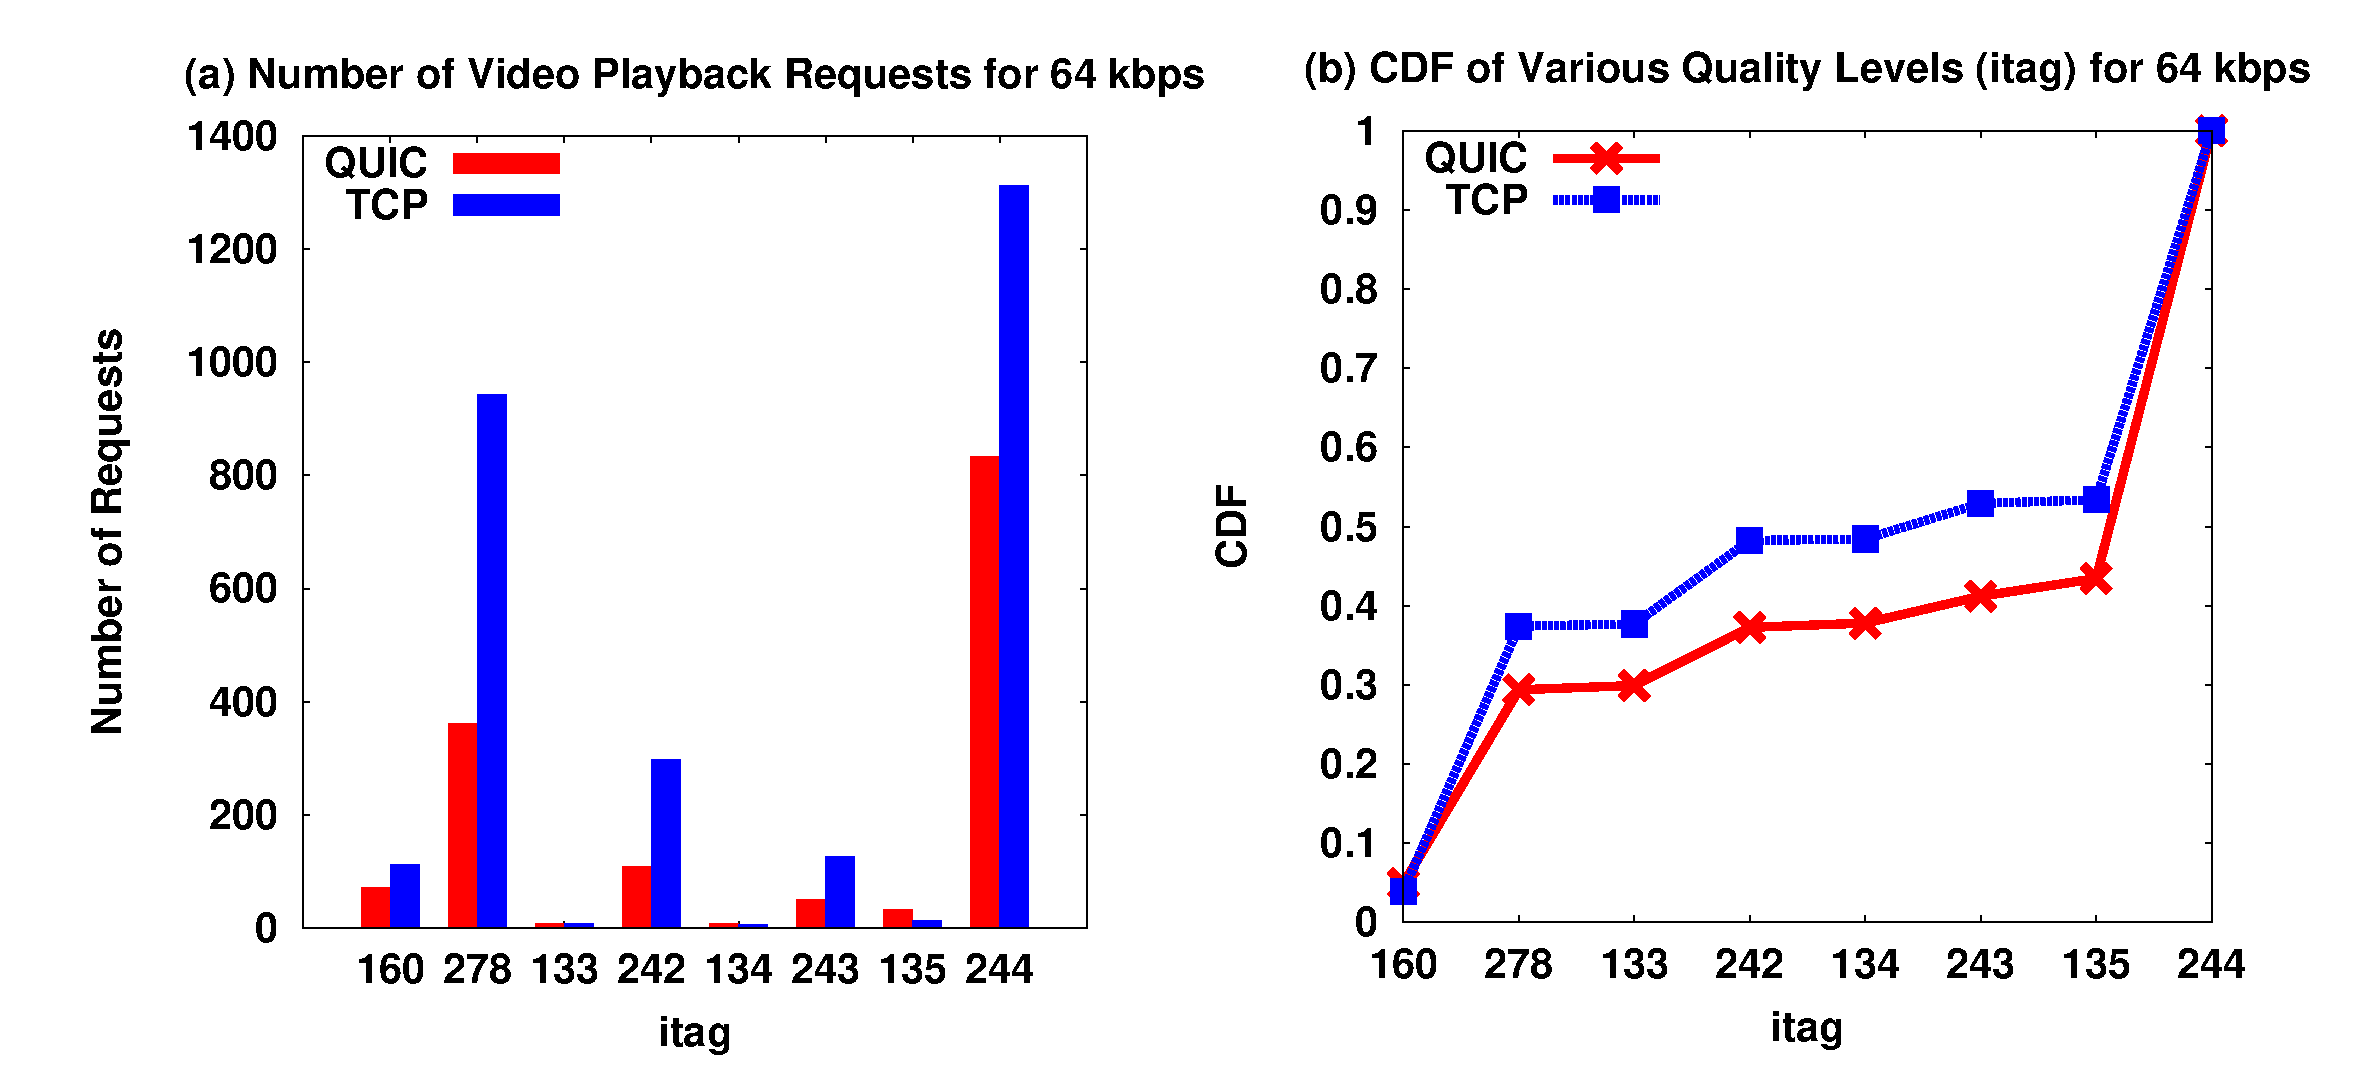
\includegraphics[width=\linewidth]{img/CDF/plot_itag_65536}
    \caption{Number of requests and CDF of itag at 64 kbps}
    \label{fig:itag6556}
\end{figure}

\begin{figure}[!ht]
    \centering
    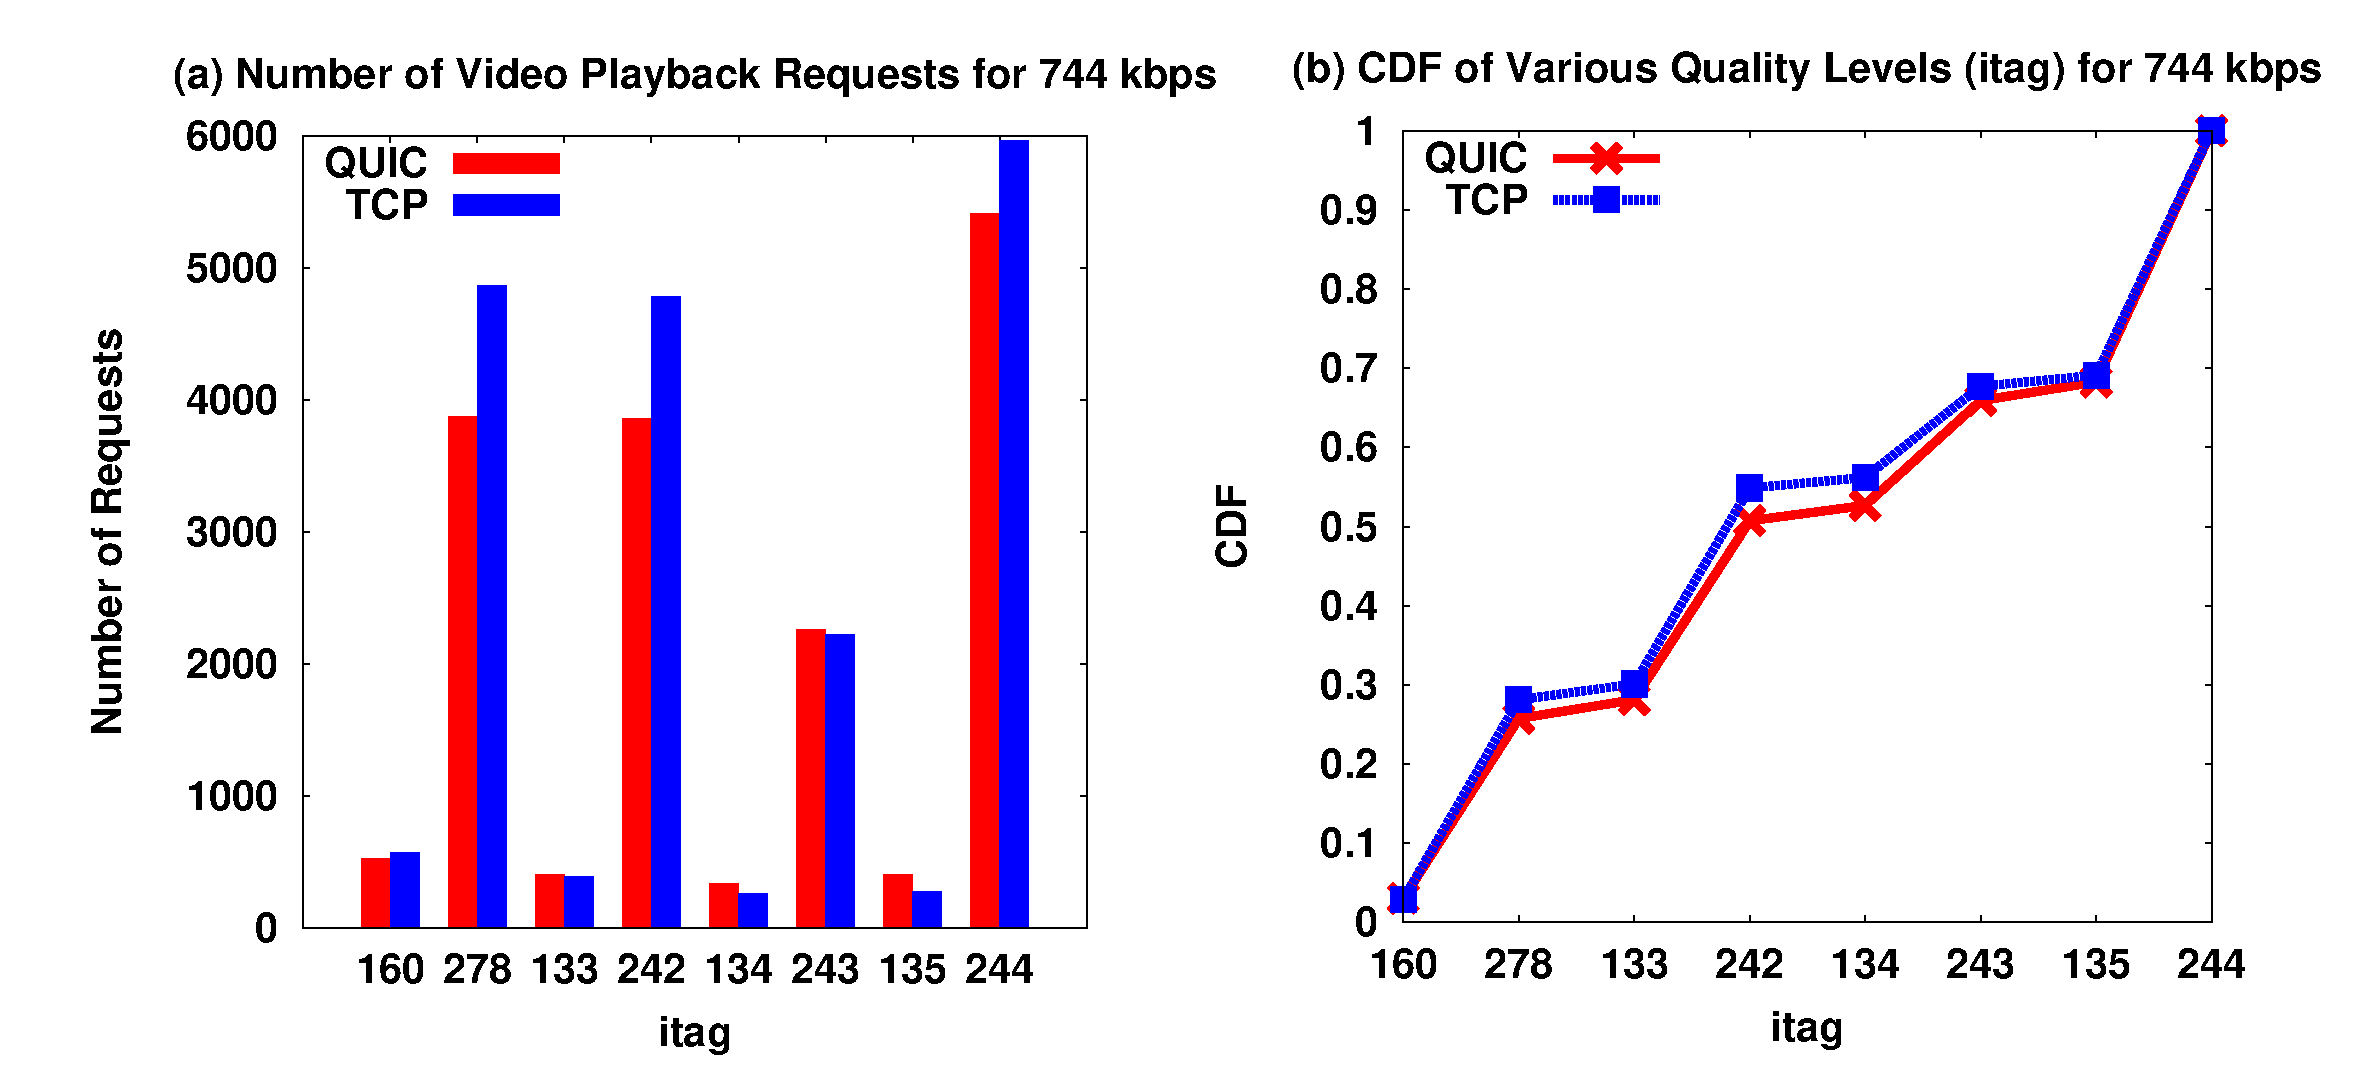
\includegraphics[width=\linewidth]{img/CDF/plot_itag_761856}
    \caption{Number of requests and CDF of itag at 744 kbps}
    \label{fig:itag761}
\end{figure}

\begin{figure}[h]
    \centering
    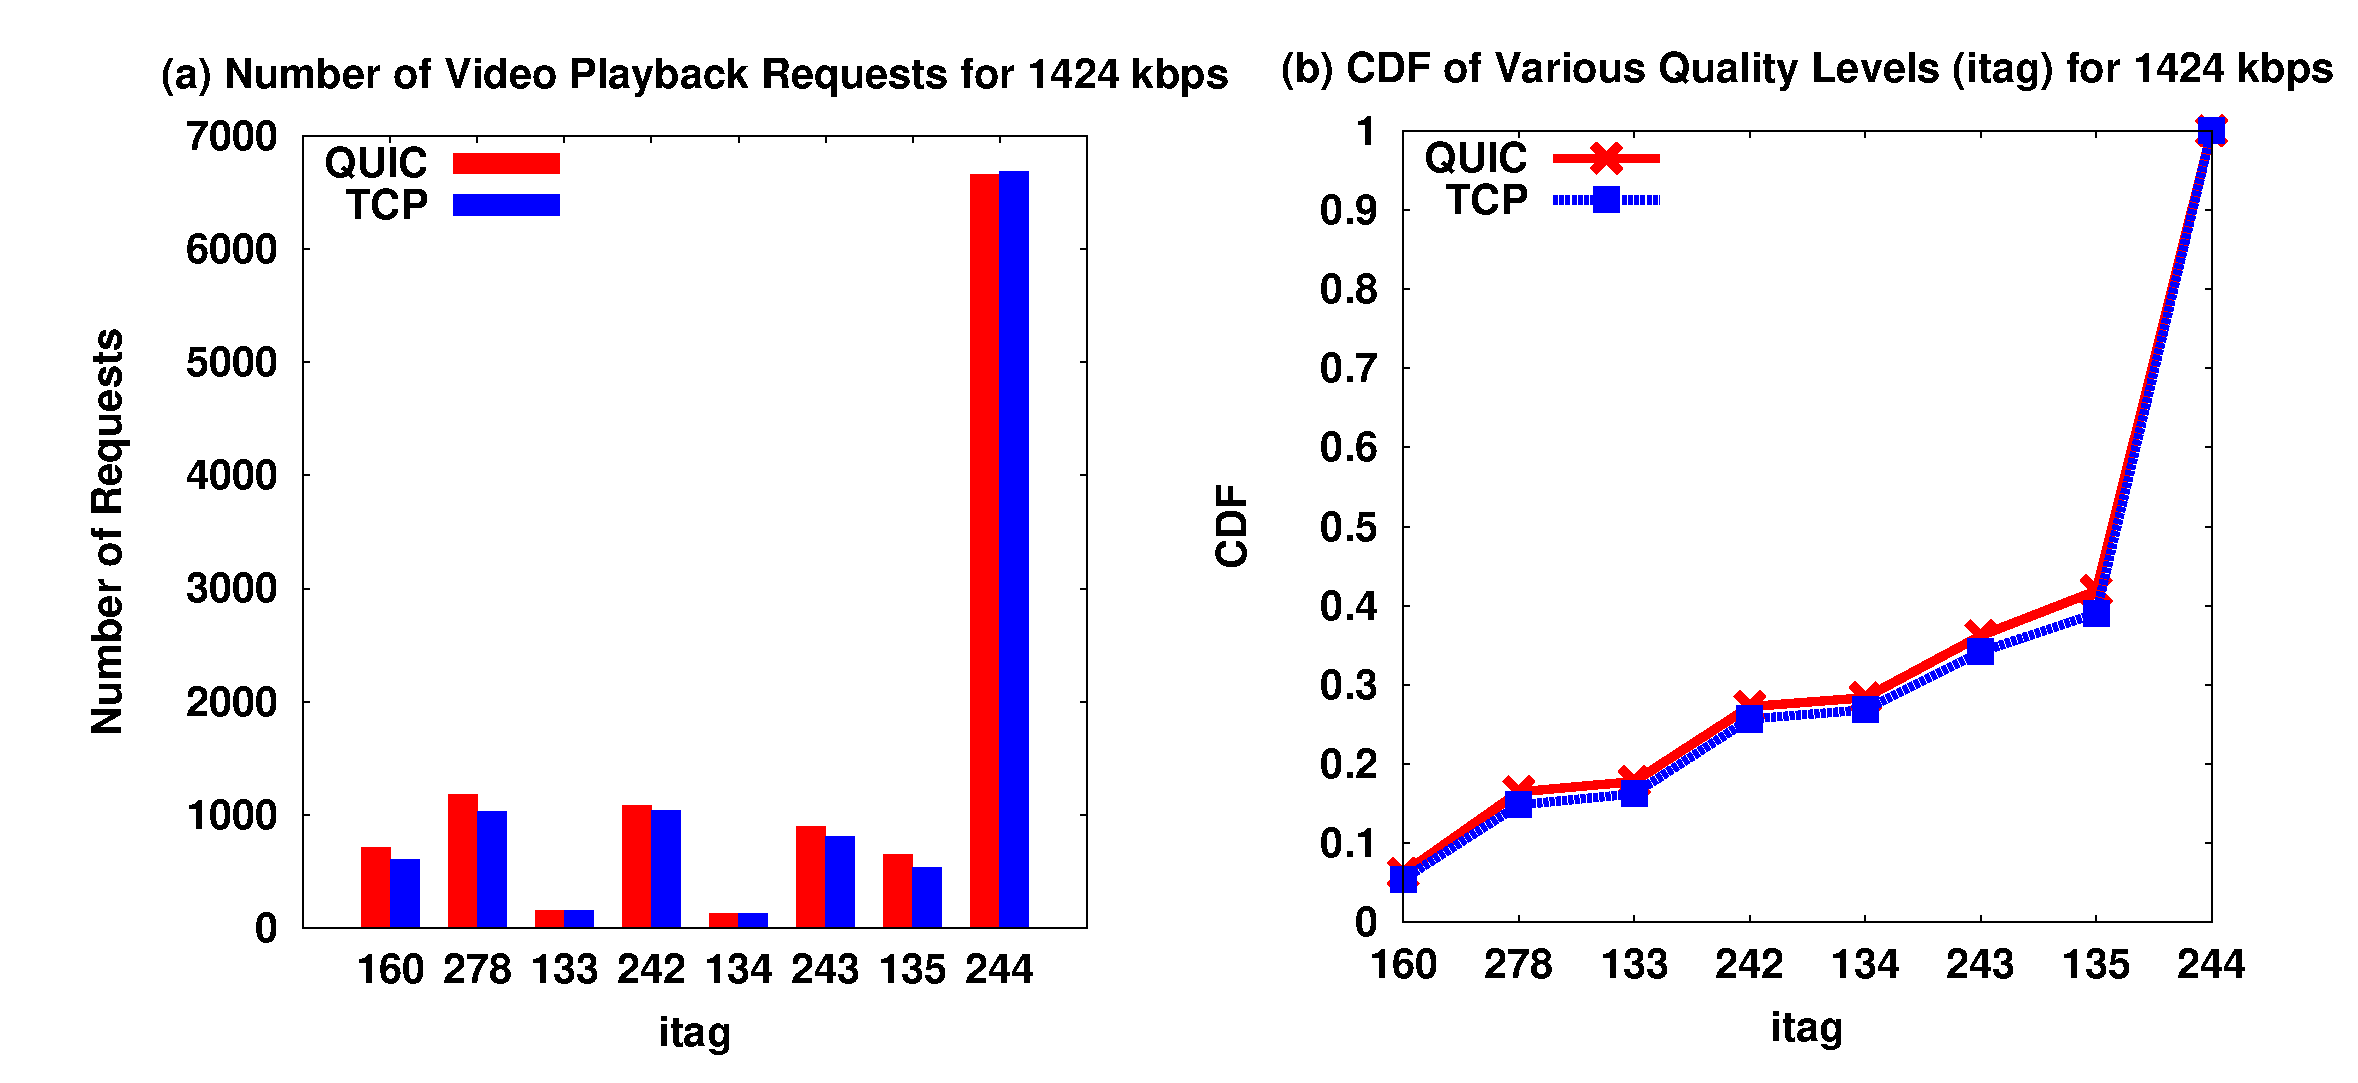
\includegraphics[width=\linewidth]{img/CDF/plot_itag_1458176}
    \caption{Number of requests and CDF of itag at 1424 kbps}
    \label{fig:itag76111}
\end{figure}

%\begin{addmargin}[2.1cm]{2.1cm}
The important observations that we can make from these CDF and number of requests plots for itag is that at lower bandwidth QUIC has higher tendency than TCP towards higher resolution but as the bandwidth increases both show similar tendencies. So at poor Internet connection speeds QUIC will provide the viewer with a better video quality than TCP. At lower speeds QUIC does not make as many requests to the server as TCP makes but at higher speeds both the protocols makes the same number of requests. This implies that QUIC is more aware of the network conditions than TCP. In the above plots when the bandwidth is at 64Kbps TCP has made almost twice the number of requests as QUIC made. This is because at 64Kbps when almost all the packets are dropped, TCP unable to quickly recognize the change in bandwidth makes the request for the same higher itag value and when they fail it makes requests for lower itags. For the total set of 175 videos the number of requests made by QUIC are lesser in number when compared to TCP which implies that QUIC requires less number of requests to serve the same or higher quality data.
%\end{addmargin}
%\restoregeometry

\subsection{CDF for \textit{rbuf} with respect to various Bandwidth levels}
\textit{rbuf} unlike \textit{itag} are a continuous domain so we won't be presenting the histogram. At higher bandwidth levels there is not much difference between the two protocols. At lower bandwidth, QUIC has greater tendency towards higher \textit{rbuf} values when compared to TCP so the buffer is emptying at a slower rate when QUIC is used. This majorly implies that the chance for buffering is lower for QUIC when compared to TCP as buffering mainly occurs at poor Internet speeds supporting the statement made by Google that there were fewer rebuffers when QUIC is used instead of TCP.


\begin{figure}[!ht]
    \centering
    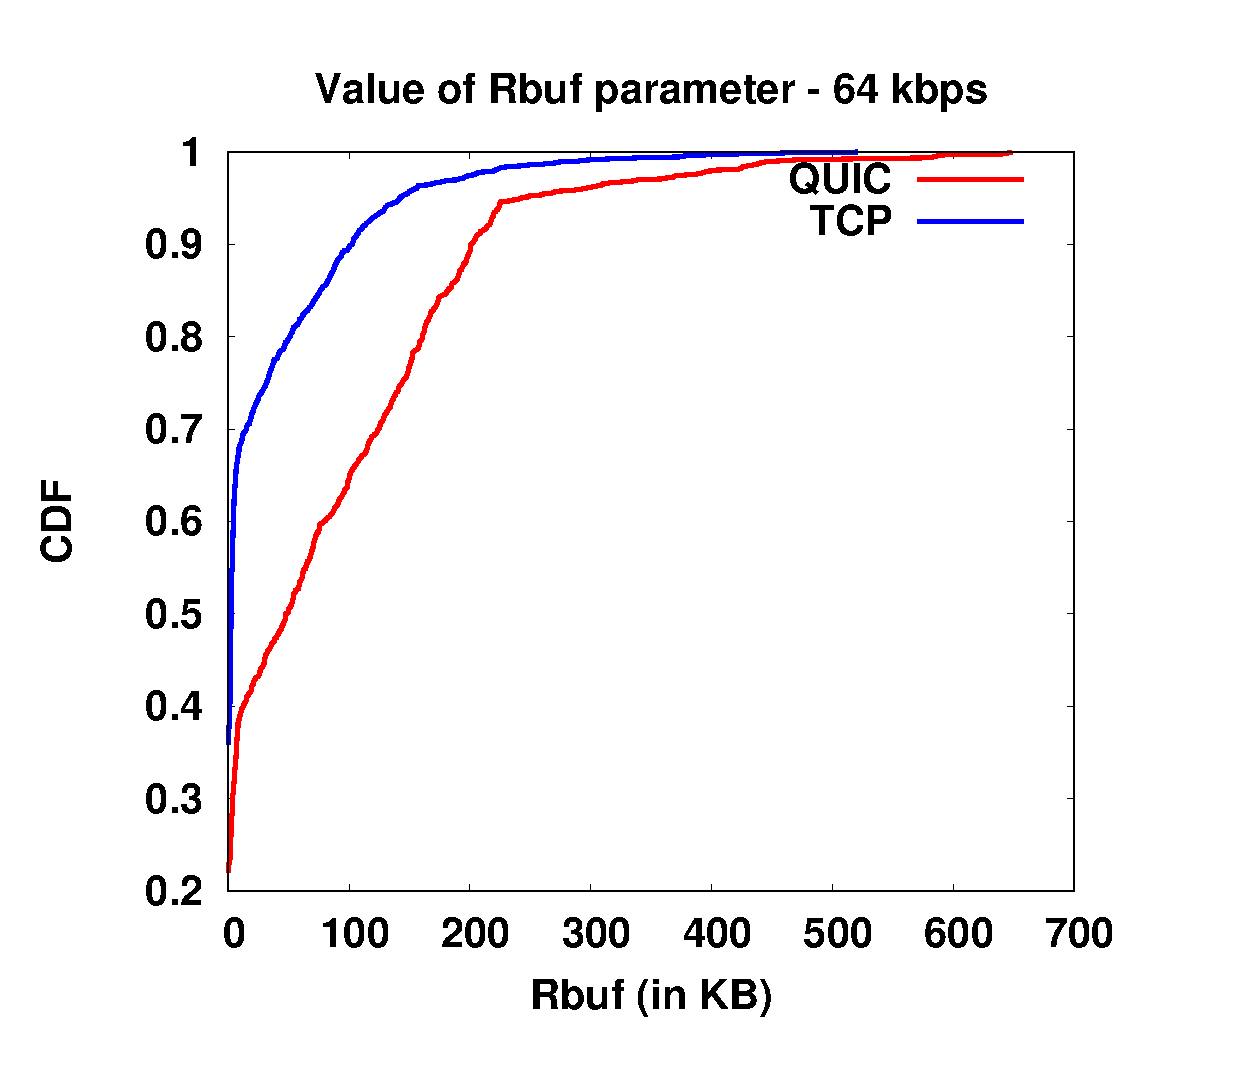
\includegraphics[width=0.9\linewidth]{img/CDF/plot_rbuf_65536}
    \caption{CDF of rbuf at 64 kbps}
    \label{fig:rbuf6556}
\end{figure}

\begin{figure}[!ht]
    \centering
    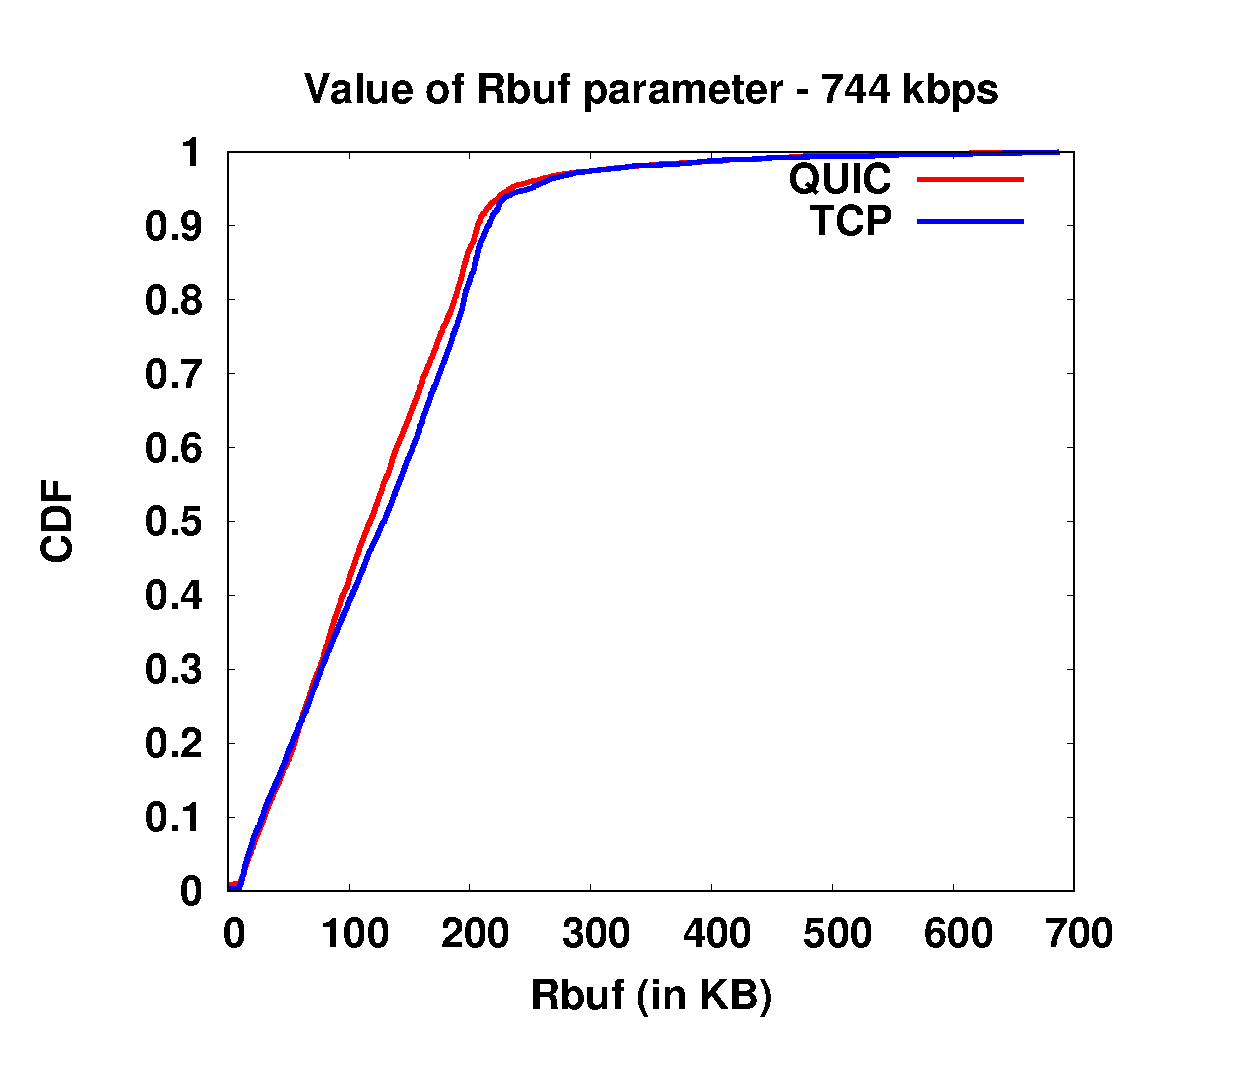
\includegraphics[width=0.9\linewidth]{img/CDF/plot_rbuf_761856}
    \caption{CDF of rbuf at 744 kbps}
    \label{fig:rbuf761856}
\end{figure}
\begin{figure}[!ht]
    \centering
    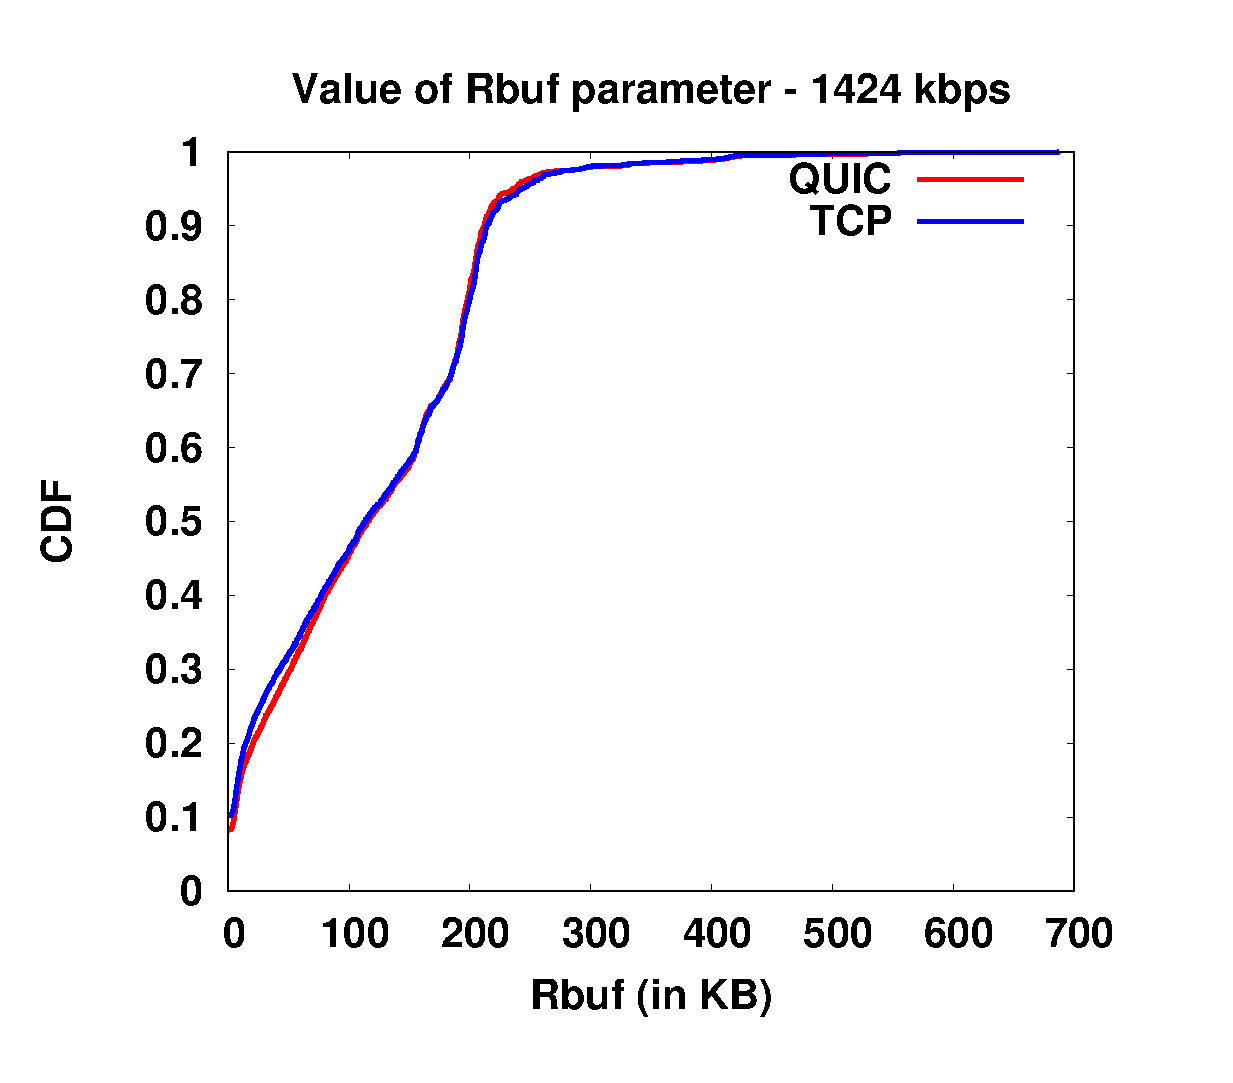
\includegraphics[width=0.9\linewidth]{img/CDF/plot_rbuf_1458176}
    \caption{CDF of rbuf at 1424 kbps}
    \label{fig:rbuf761}
\end{figure}



\subsection{CDF for \textit{range} with respect to various Bandwidth levels}
As described earlier \textit{range} parameter consists of two values separated by a \\dash (-) and they define the byte range of the video for a itag value that the client requests from the server. We have taken the difference between these two values and plotted the CDF plots. At higher bandwidth levels the two protocols doesn't differ but at lower bandwidth QUIC has a greater tendency to request data in larger chunks when compared to TCP. Since QUIC is requesting in larger chunks we can estimate that it requires lesser number of requests to server to fetch data which is confirmed by the Fig. 3.8-3.10.

\begin{figure}[!ht]
    \centering
    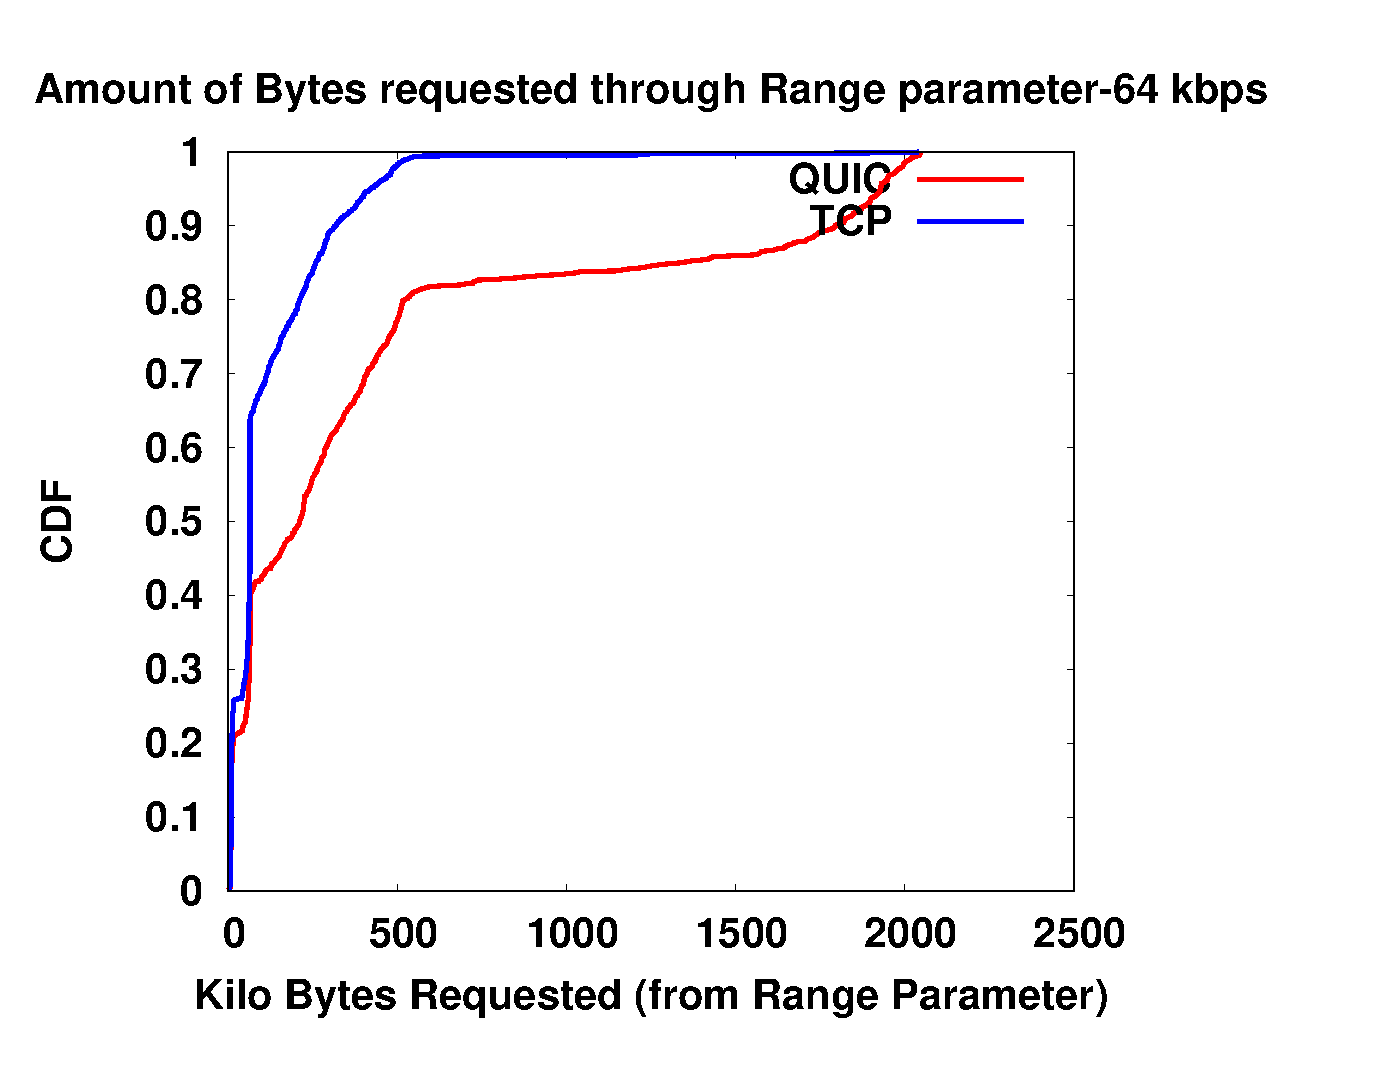
\includegraphics[width=0.9\linewidth]{img/CDF/plot_range_65536}
    \caption{CDF of range at 64 kbps}
    \label{fig:range6556}
\end{figure}
\begin{figure}[!ht]
    \centering
    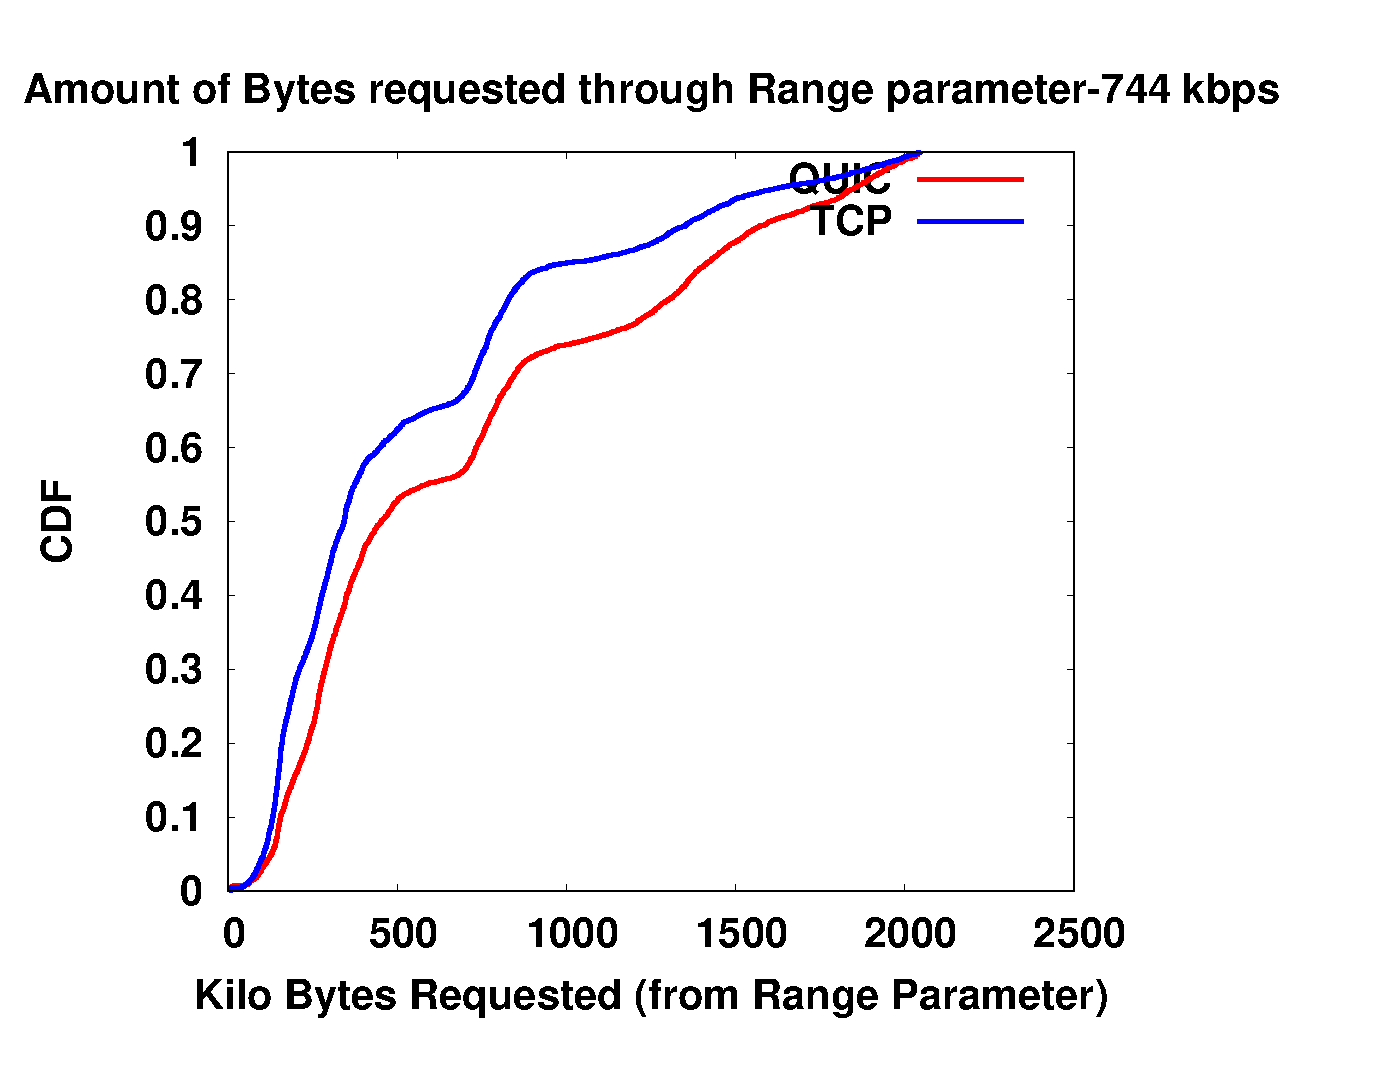
\includegraphics[width=0.9\linewidth]{img/CDF/plot_range_761856}
    \caption{CDF of range at 744 kbps}
    \label{fig:rang4761}
\end{figure}
\begin{figure}[!ht]
    \centering
    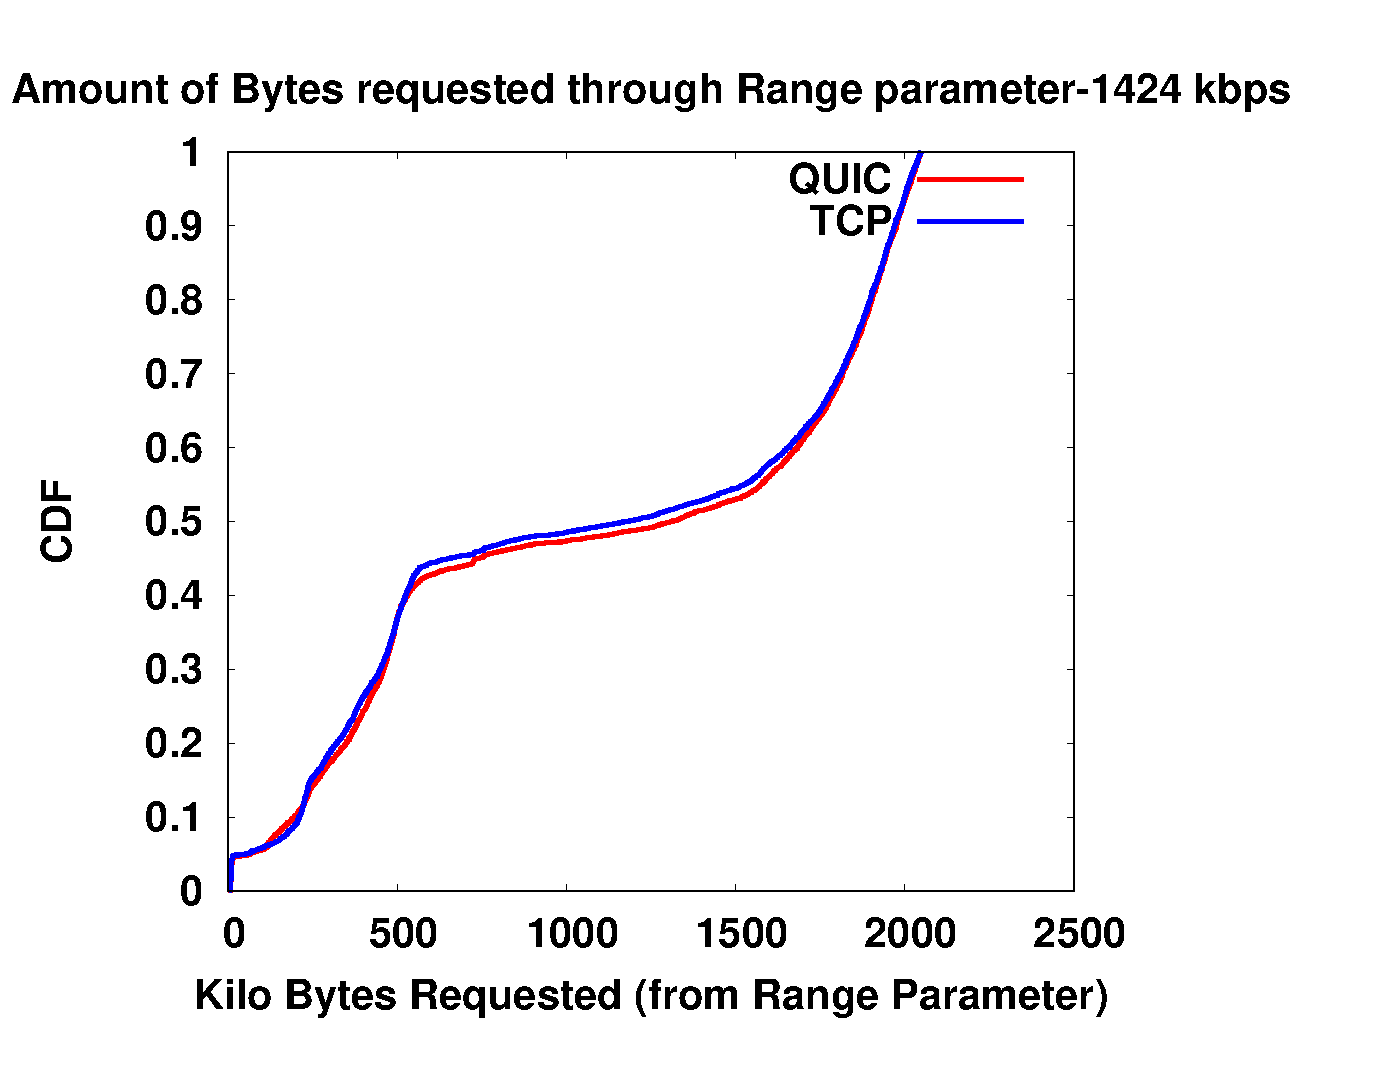
\includegraphics[width=0.9\linewidth]{img/CDF/plot_range_1458176}
    \caption{CDF of range at 1424 kbps}
    \label{fig:rang761}
\end{figure}

\subsection{CDF for Segment Length with respect to various Bandwidth levels}
This is another way of representing the \textit{range} parameter. From the number of bytes requested through range parameter we can convert it into duration of playback seconds using the bit-rates for the \textit{itags}. The trends will be similar to the CDF plots of \textit{range} with QUIC trying to request segments with longer duration when compared to TCP at lower bandwidths but at higher bandwidths the difference is not much.

\begin{figure}[!ht]
    \centering
    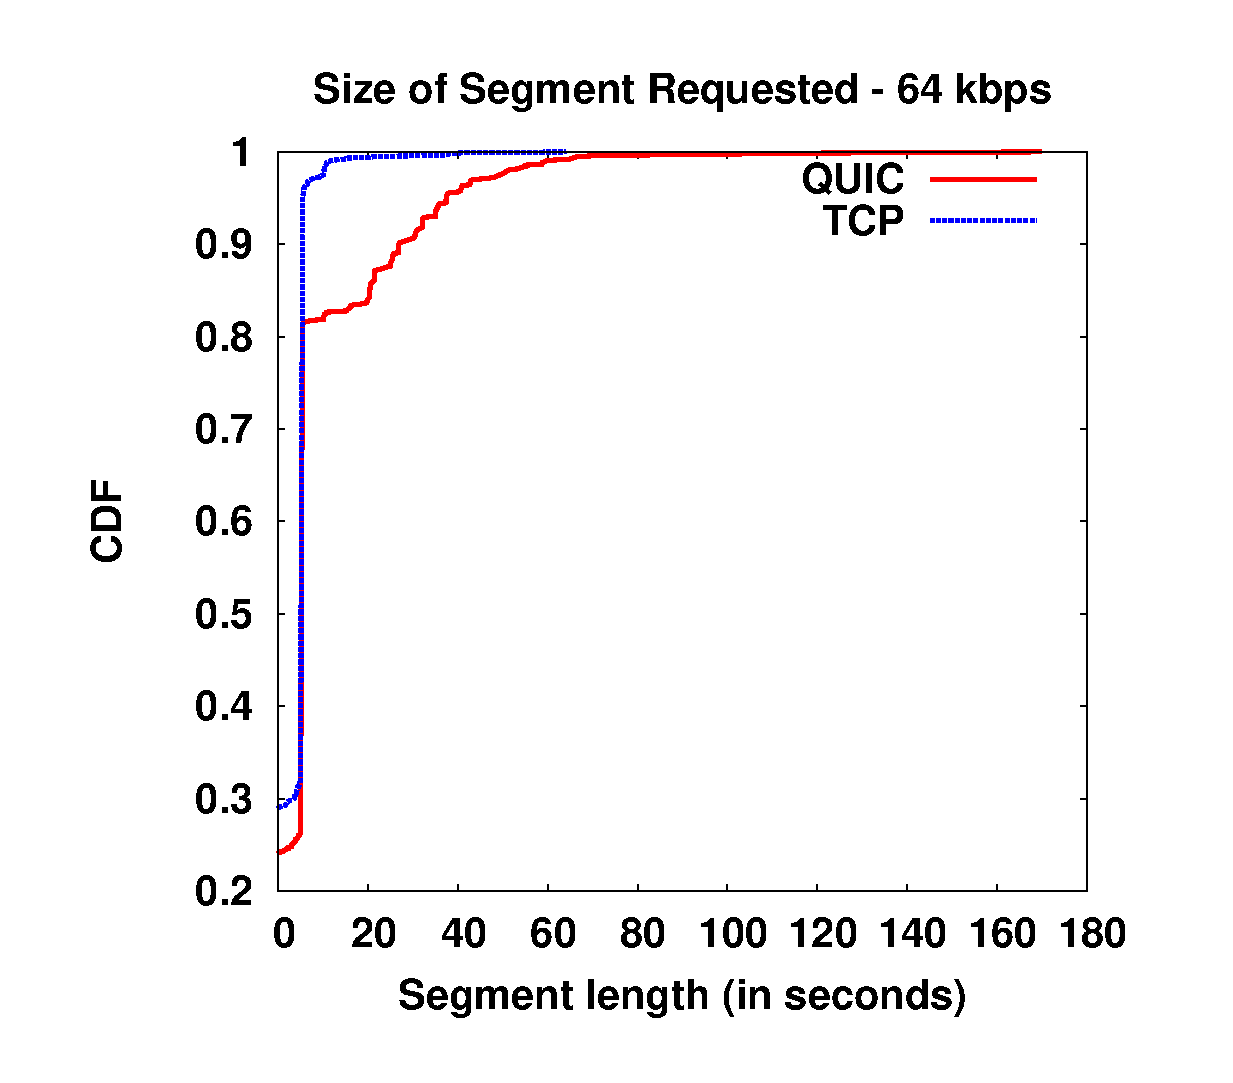
\includegraphics[width=0.9\linewidth]{img/CDF/plot_segment_65536}
    \caption{CDF of Segment Length at 64 kbps}
    \label{fig:seg6556}
\end{figure}
\begin{figure}[!ht]
    \centering
    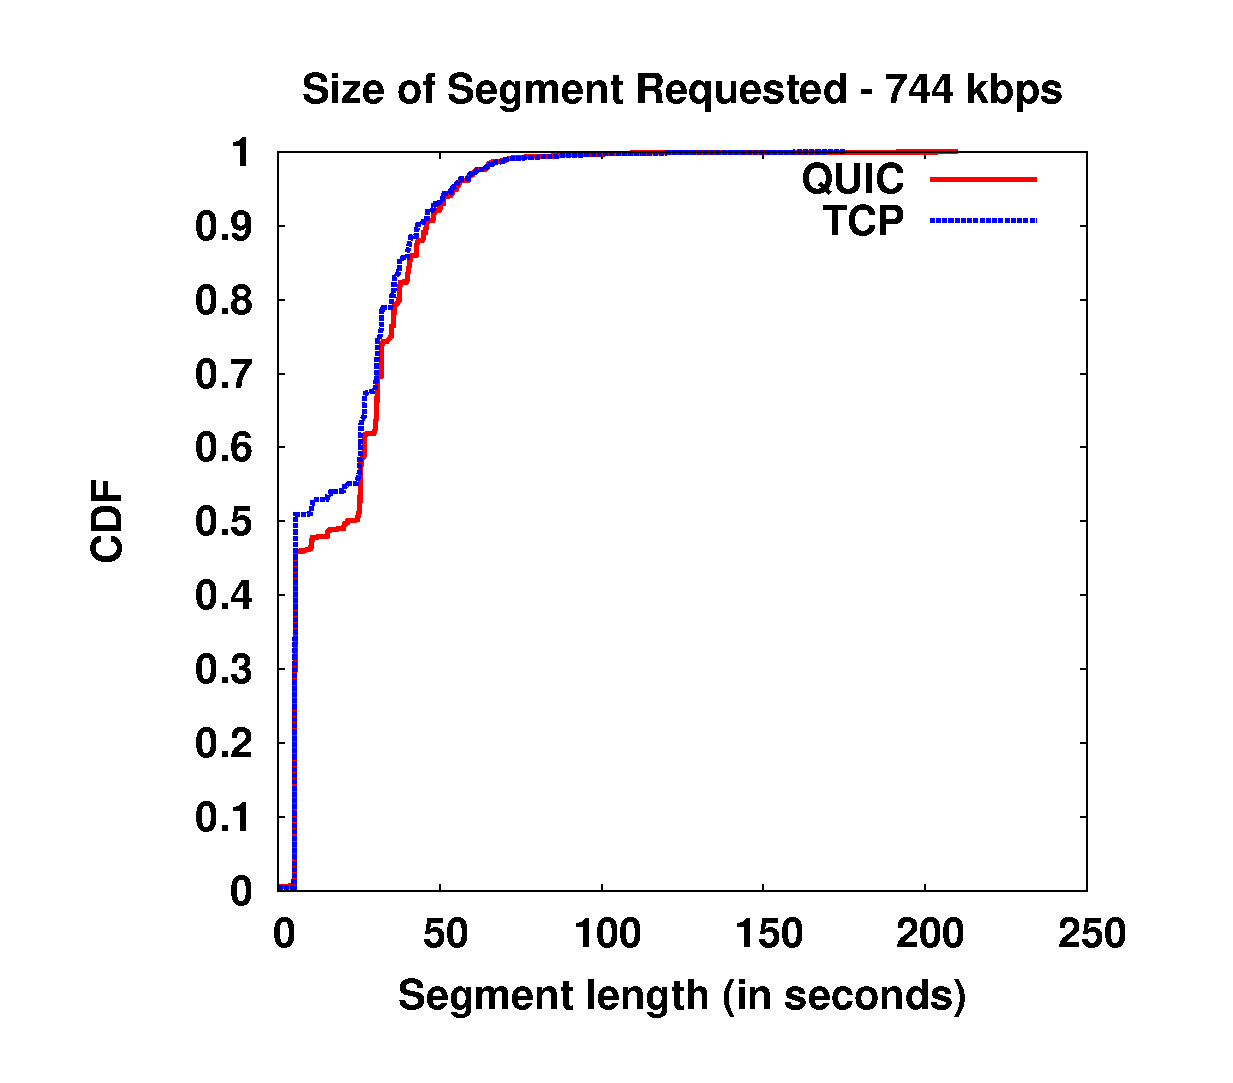
\includegraphics[width=0.9\linewidth]{img/CDF/plot_segment_761856}
    \caption{CDF of Segment Length at 744 kbps}
    \label{fig:seg7621}
\end{figure}
\begin{figure}[!ht]
    \centering
    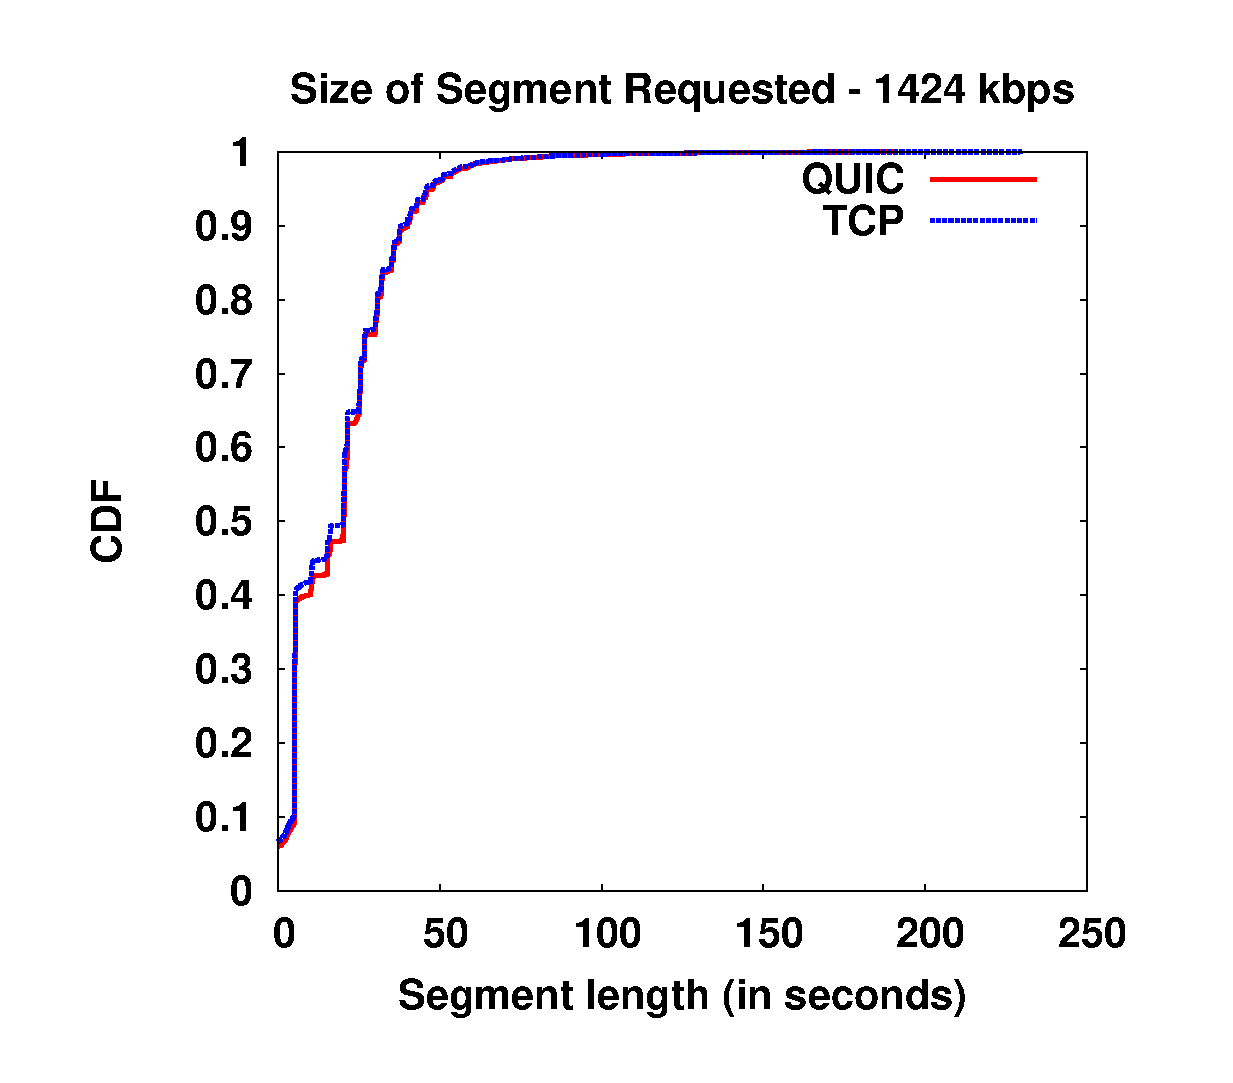
\includegraphics[width=0.9\linewidth]{img/CDF/plot_segment_1458176}
    \caption{CDF of Segment Length at 1424 kbps}
    \label{fig:seg761}
\end{figure}


%\begin{addmargin}[2.1cm]{2.1cm}
\subsection{CDF for \textit{itag} with respect to various \textit{rbuf} ranges(buckets) }
The two protocols does not differ much with respect to \textit{rbuf}. When the buffer is smaller in amount they fetch all the itags but when the buffer is sufficiently large both the protocols fetch data only for higher itags as it is evident in the last two plots. QUIC makes more number of requests than TCP when the client has buffered large amount of data. This can be interpreted as QUIC's estimation that since buffer has large amount of data the rate of data consumption is less when compared to data fetched so bandwidth is sufficiently good and it can make further requests. It is also evident that most of the requests to server were made when the buffer is low in data as both the protocols interpret this as data depletion at a faster rate so they try to fetch data at a faster rate which means more number of requests made.

%\end{addmargin}

\begin{figure}[!ht]
    \centering
    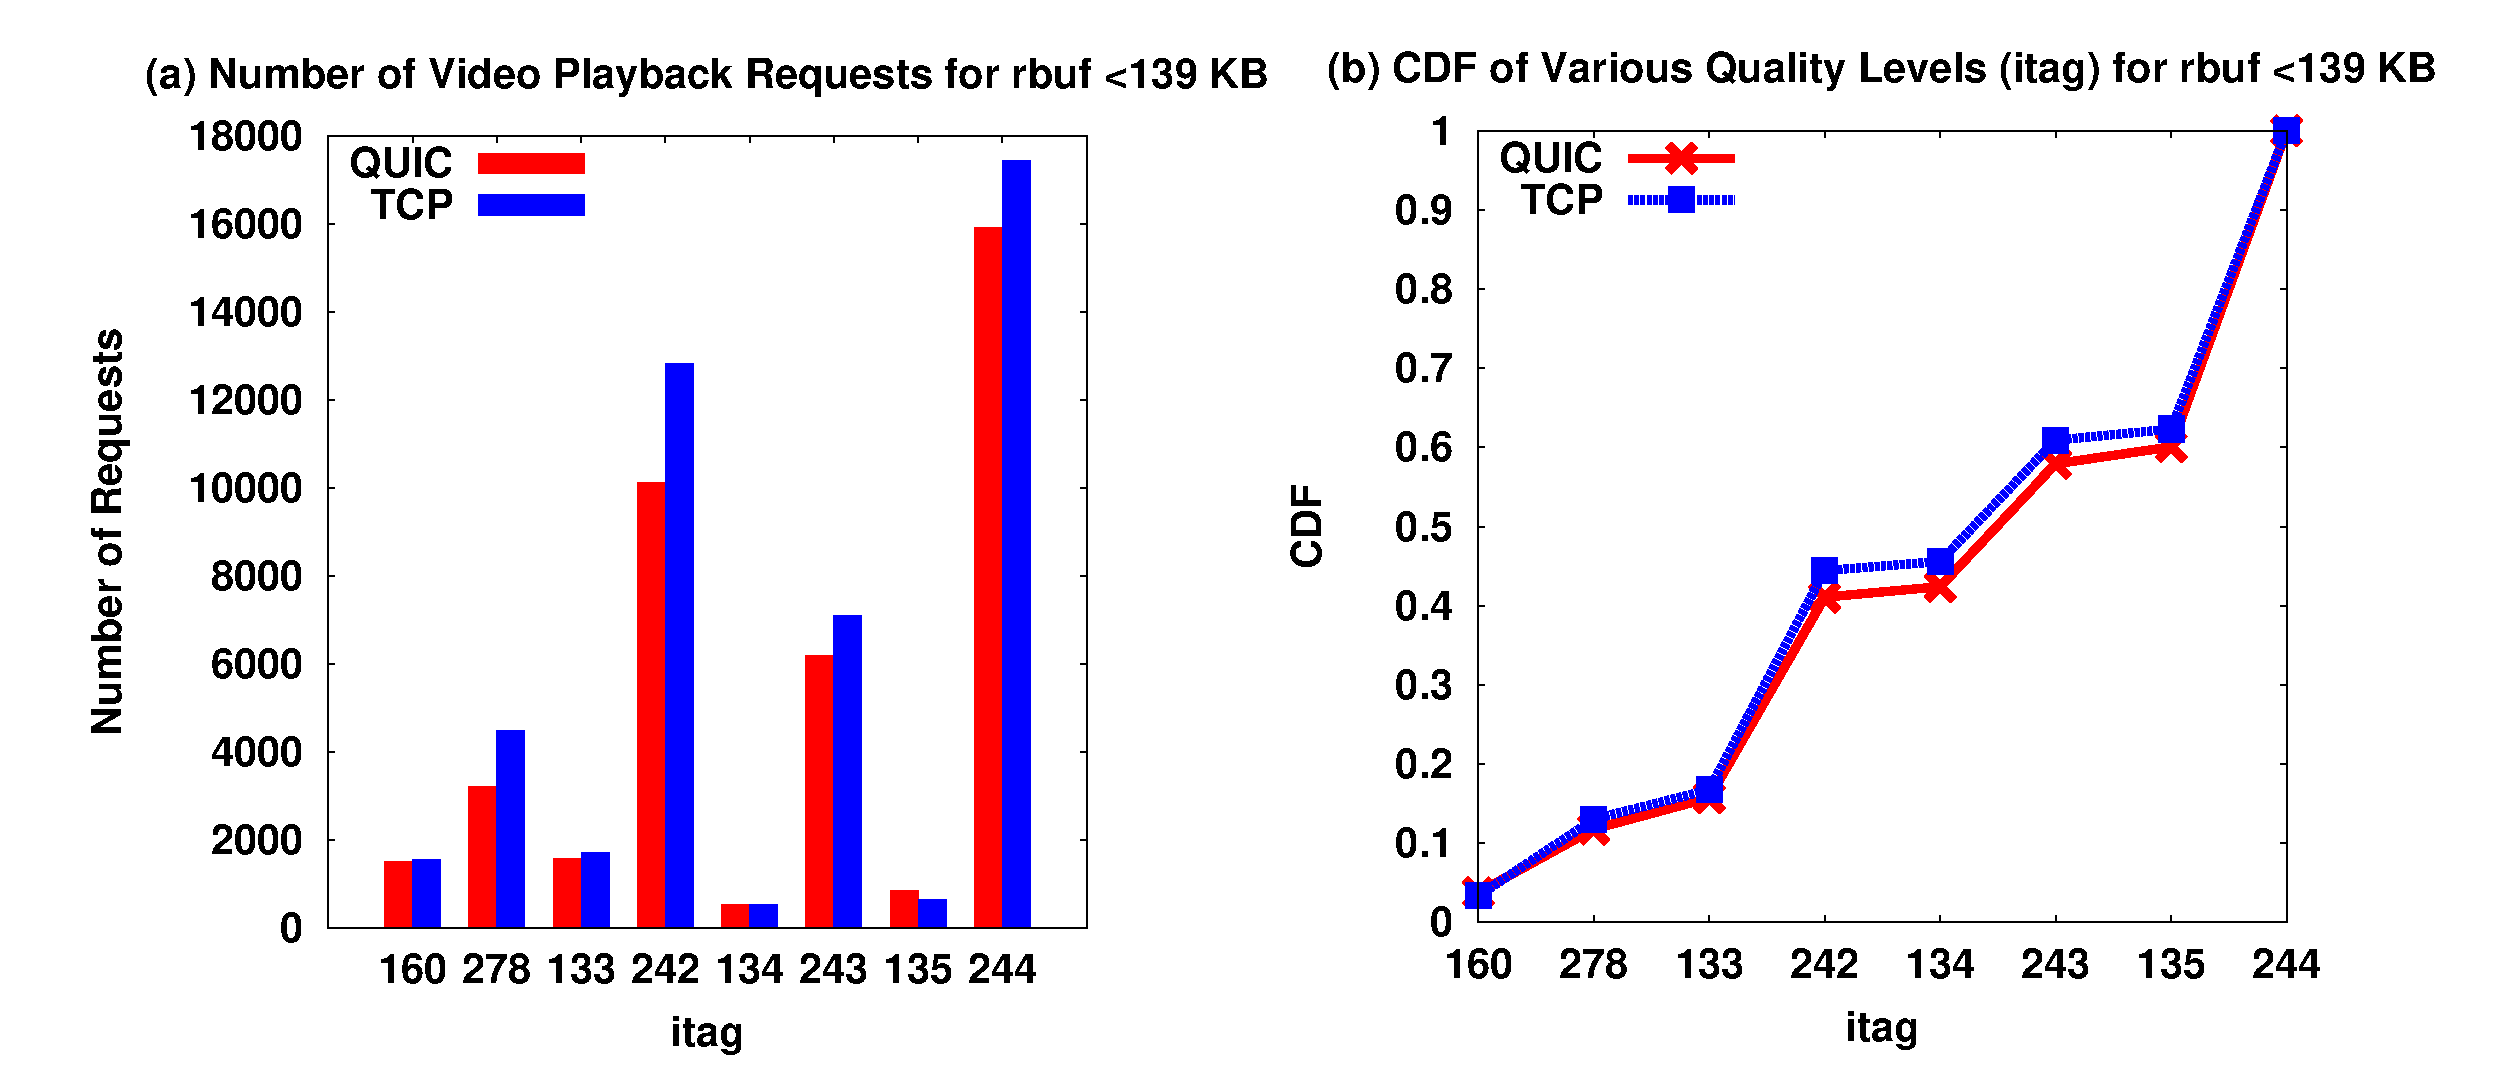
\includegraphics[width=0.9\linewidth]{img/CDF/plot_itag_142367}
    \caption{Number of requests and CDF of itag for rbuf $<$139 KB}
    \label{fig:itag761121}
\end{figure}

\begin{figure}[!ht]
    \centering
    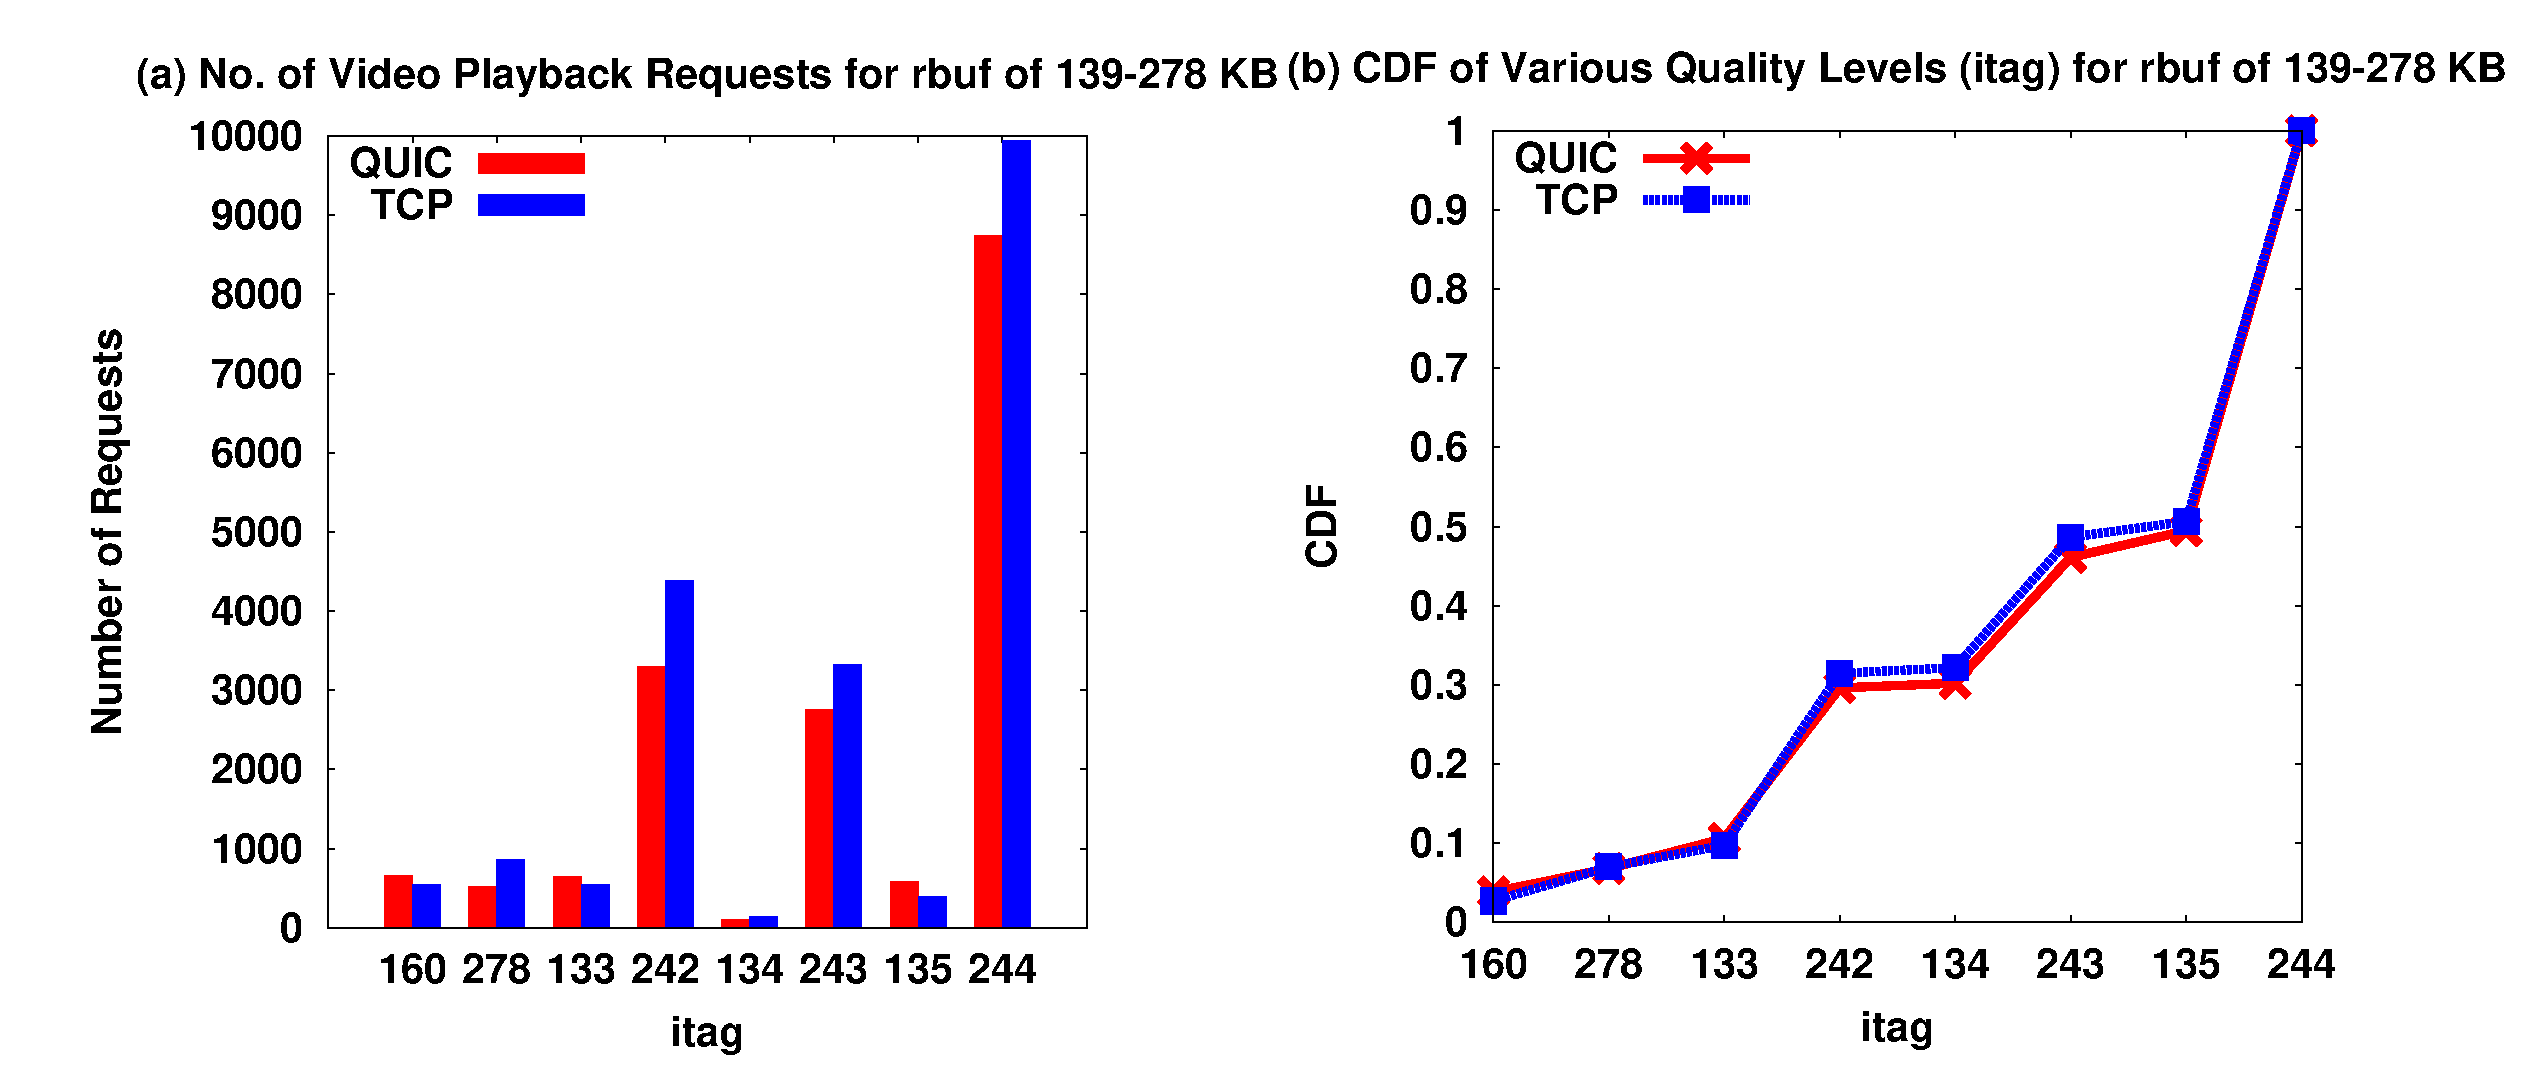
\includegraphics[width=0.9\linewidth]{img/CDF/plot_itag_284734}
    \caption{Number of requests and CDF of itag for rbuf 139-278 KB}
    \label{fig:itag65526}
\end{figure}
\begin{figure}[!ht]
    \centering
    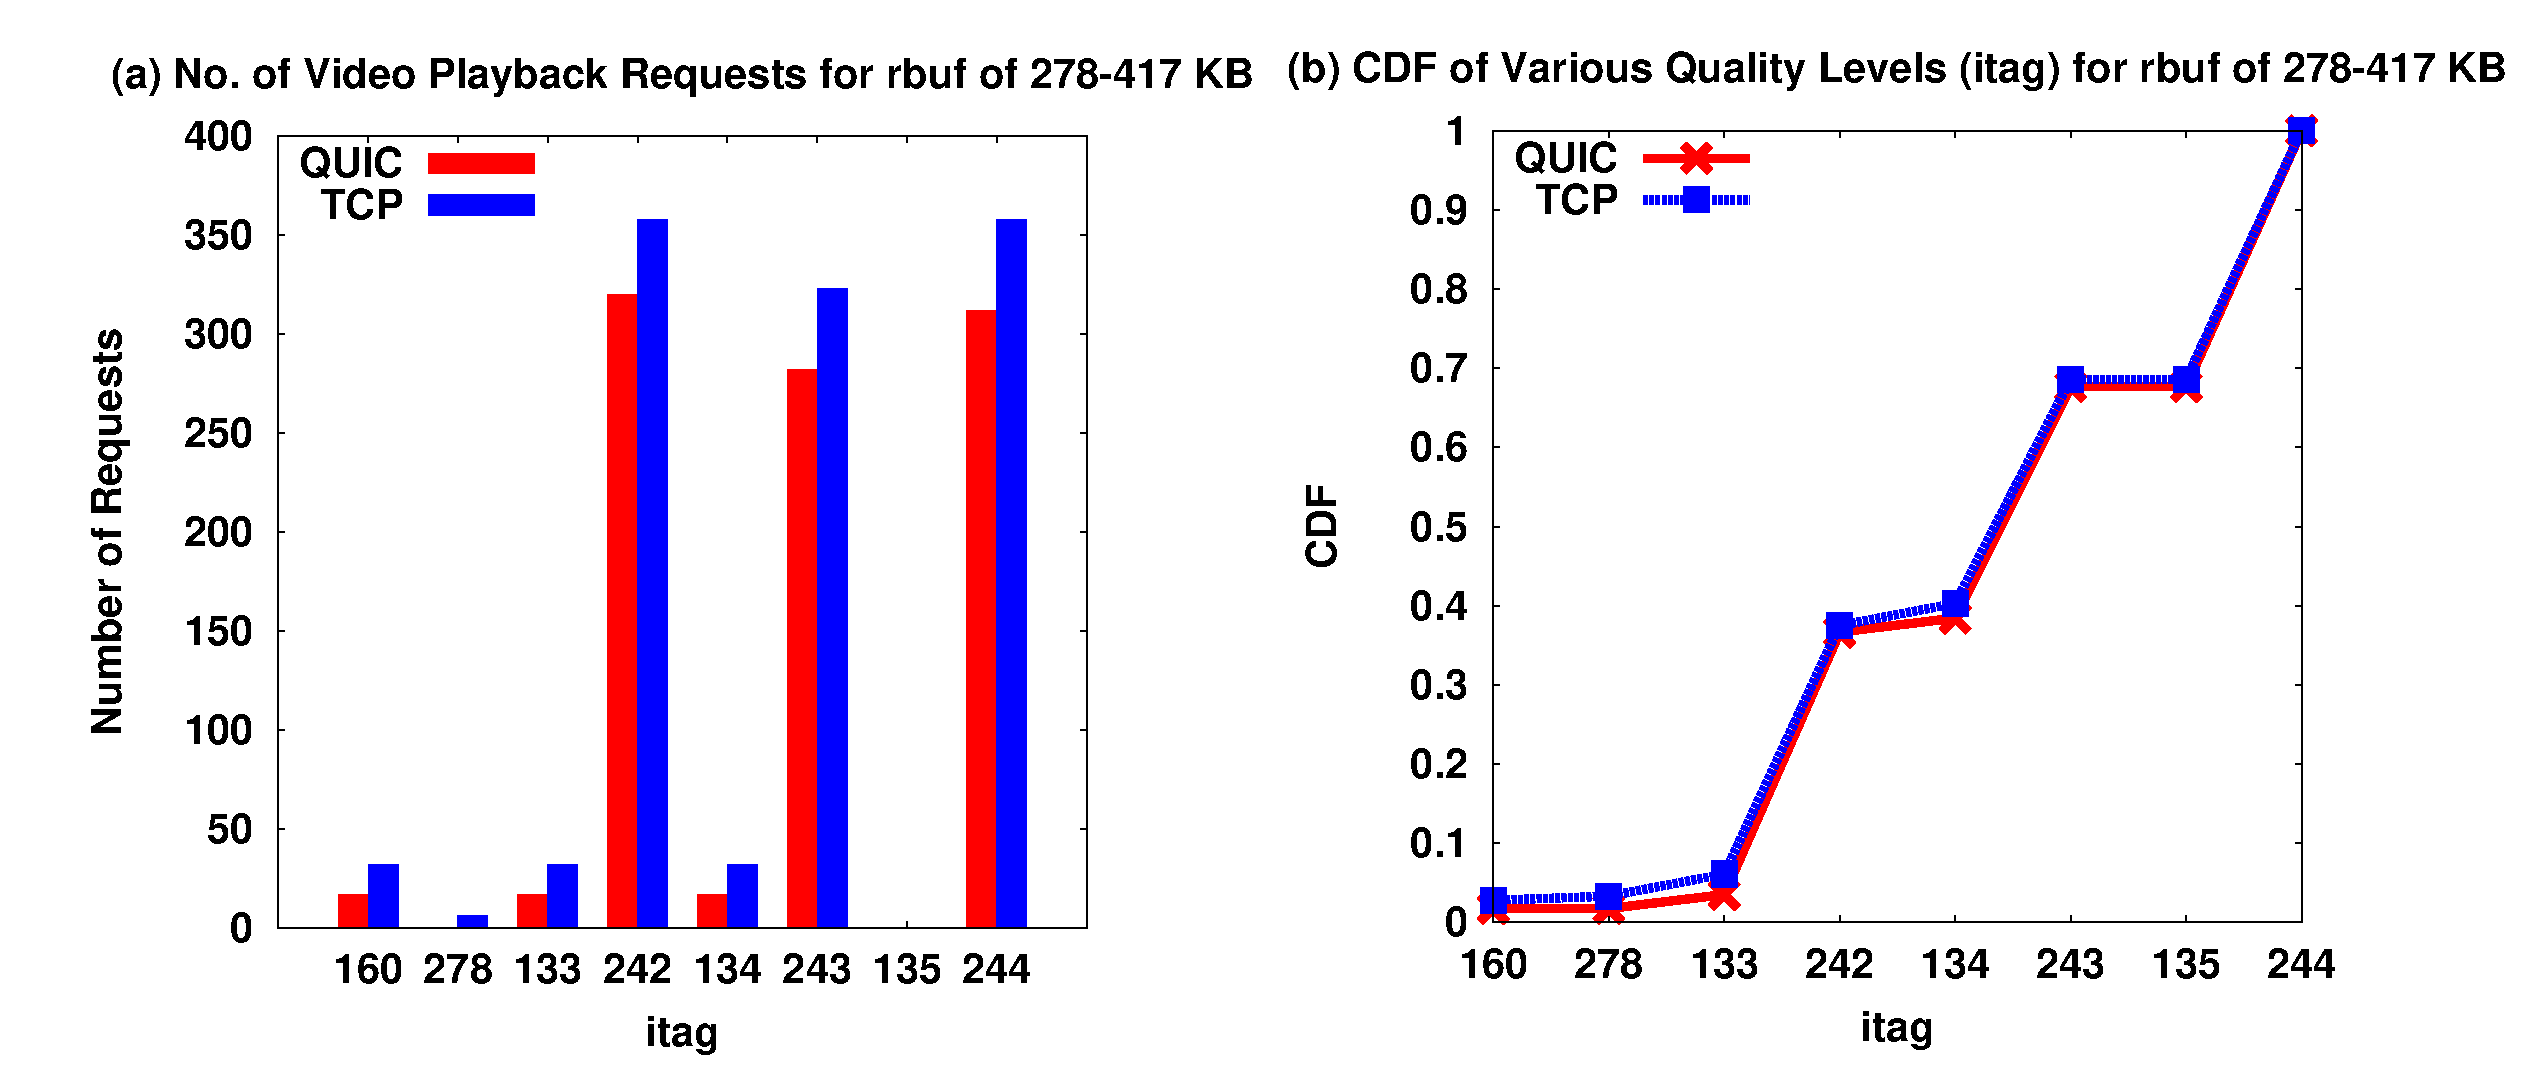
\includegraphics[width=0.9\linewidth]{img/CDF/plot_itag_427101}
    \caption{Number of requests and CDF of itag for rbuf 278-417 KB}
    \label{fig:itag7612}
\end{figure}

\begin{figure}[!ht]
    \centering
    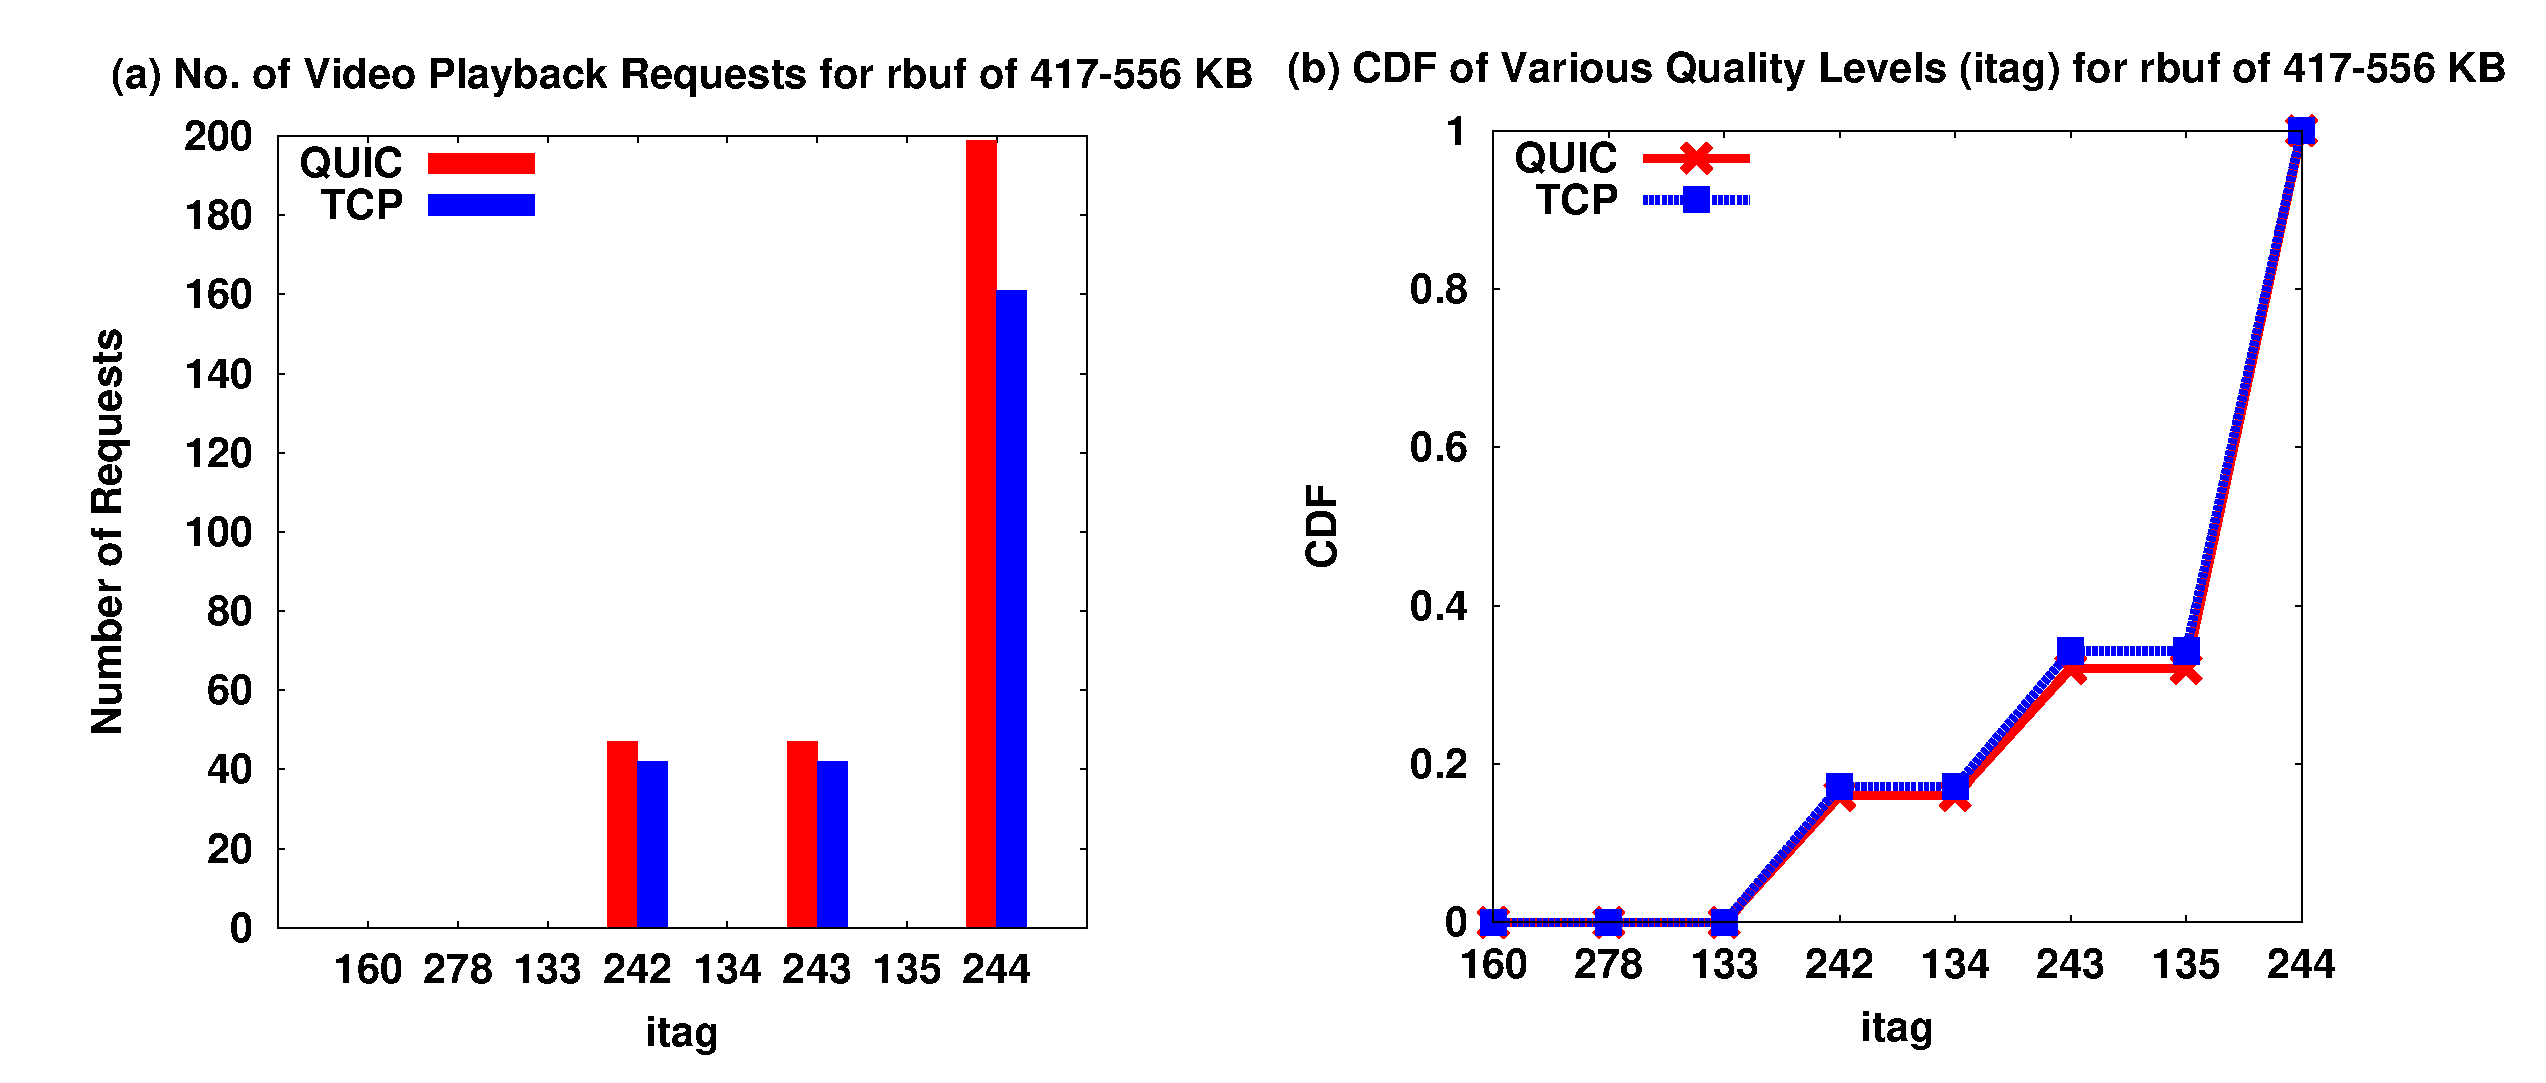
\includegraphics[width=0.9\linewidth]{img/CDF/plot_itag_569468}
    \caption{Number of requests and CDF of itag for rbuf 417-556 KB}
    \label{fig:itag65561}
\end{figure}
\begin{figure}[!ht]
    \centering
    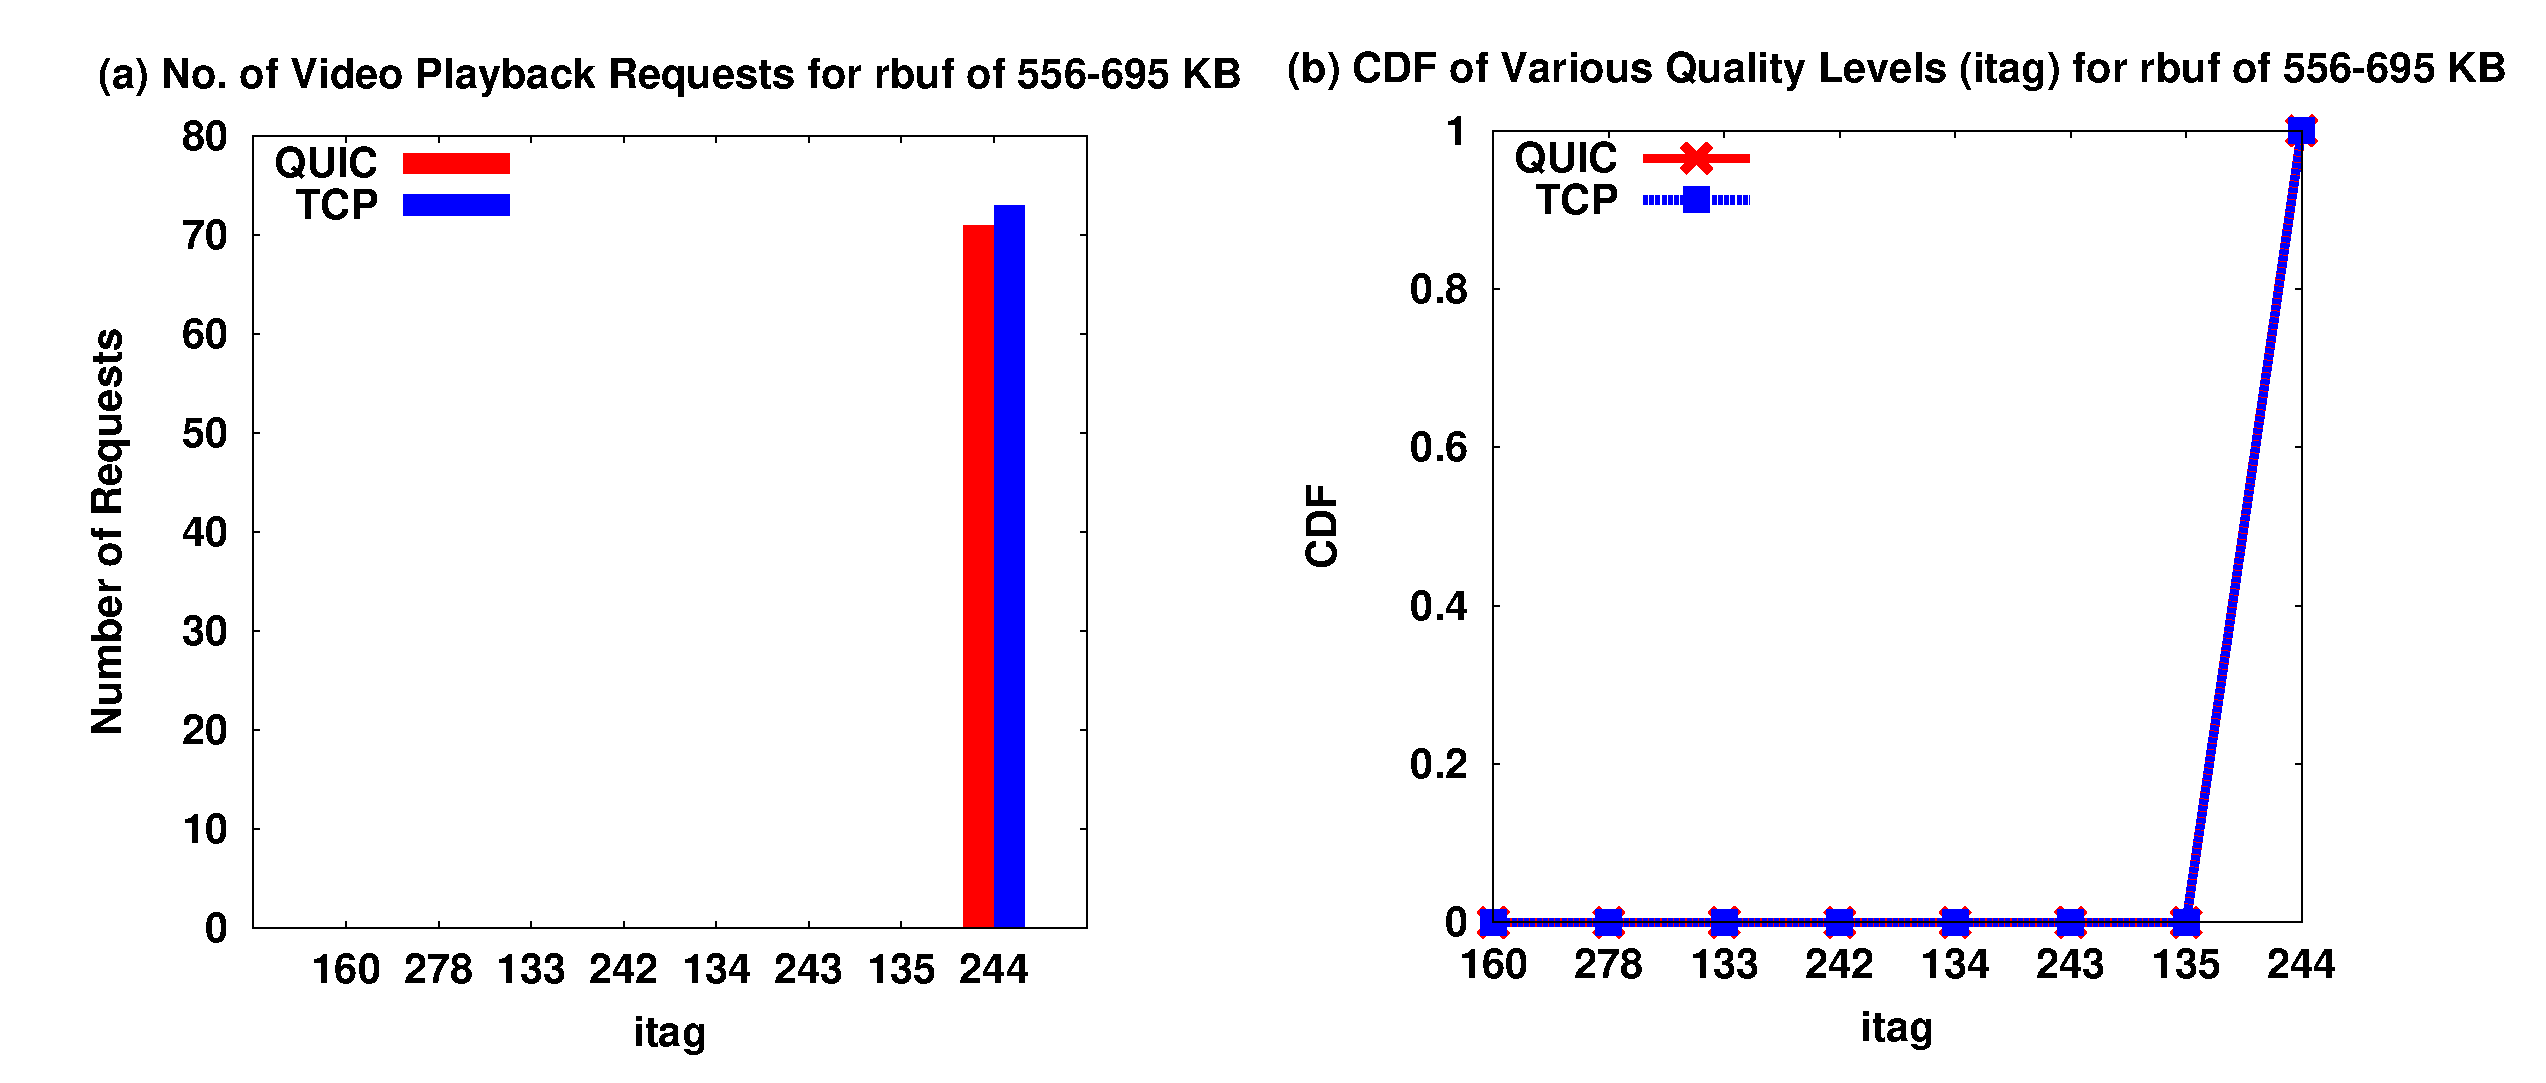
\includegraphics[width=0.9\linewidth]{img/CDF/plot_itag_711837}
    \caption{Number of requests and CDF of itag for rbuf 556-695 KB}
    \label{fig:itag7611}
\end{figure}

\subsection{CDF for \textit{range} with respect to various \textit{rbuf} ranges(buckets) }
The behaviour of both the protocols is similar when the buffer is quite low or quite high but when the buffer is in the medium range QUIC and TCP show a different pattern. When the buffer is low both the protocols take a conservative approach and request the data in smaller chunks but QUIC requests the data in a slightly larger chunks. When the buffer is above a threshold value QUIC and TCP differ in that QUIC tries to download the data in larger chunks when compared to TCP. When the buffer is sufficiently high both the protocols doesn't differ much.
\begin{figure}[!ht]
    \centering
    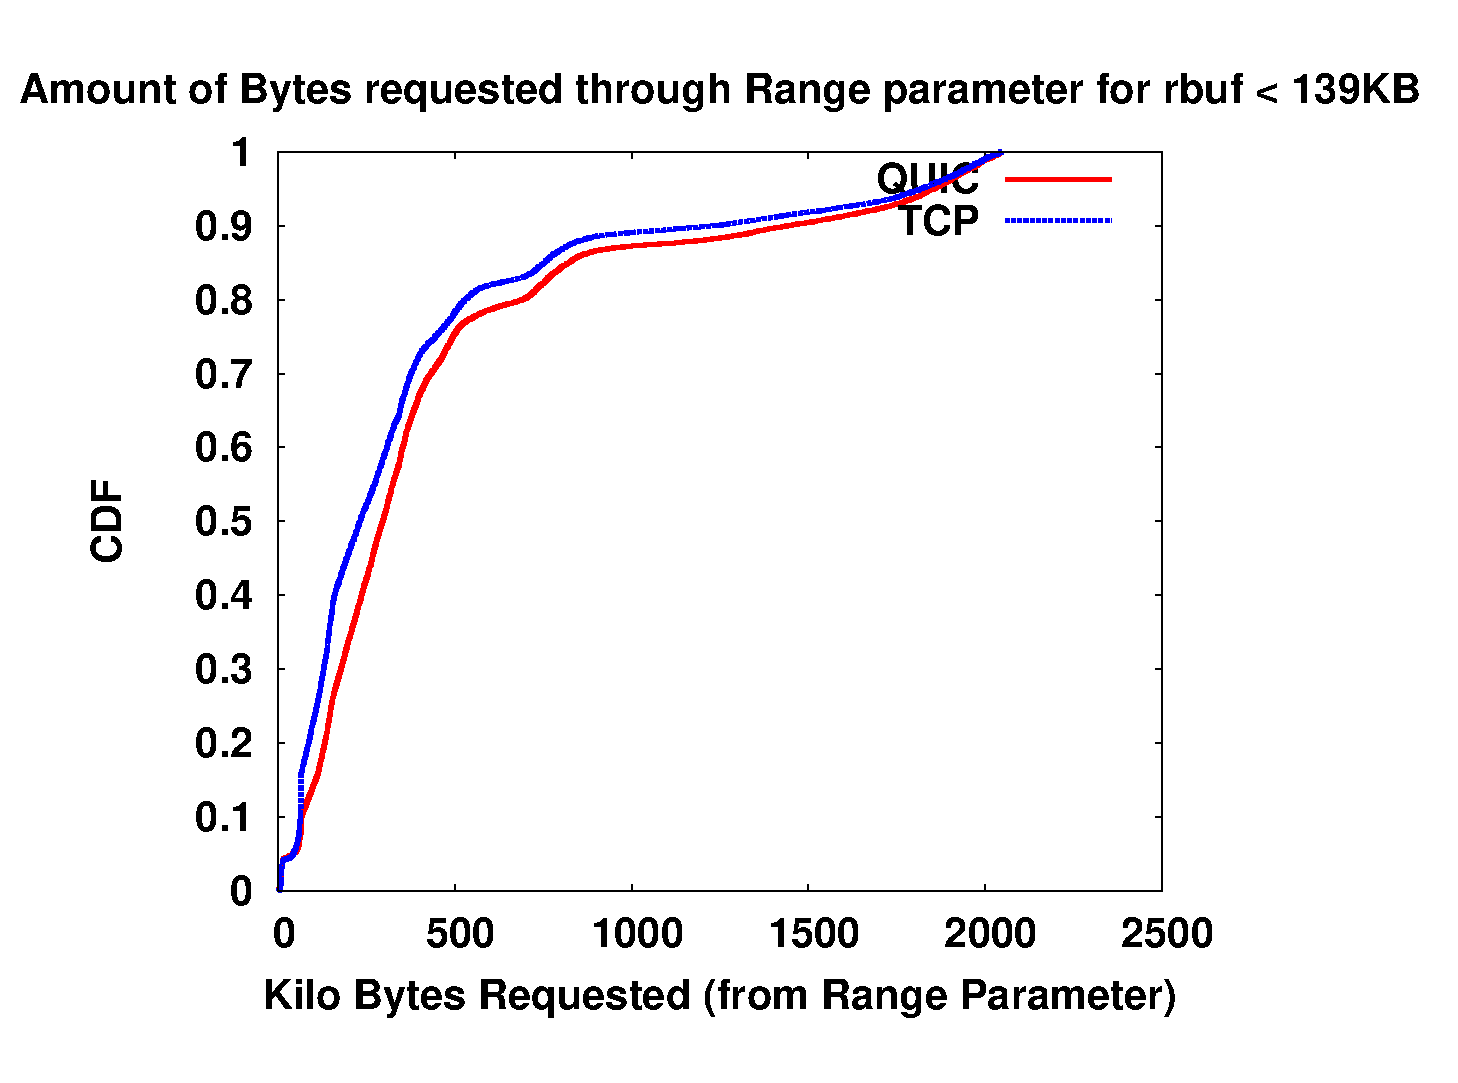
\includegraphics[width=0.9\linewidth]{img/CDF/plot_range_142367}
    \caption{CDF of range for rbuf $<$ 139KB}
    \label{fig:rabuf6556}
\end{figure}

\begin{figure}[!ht]
    \centering
    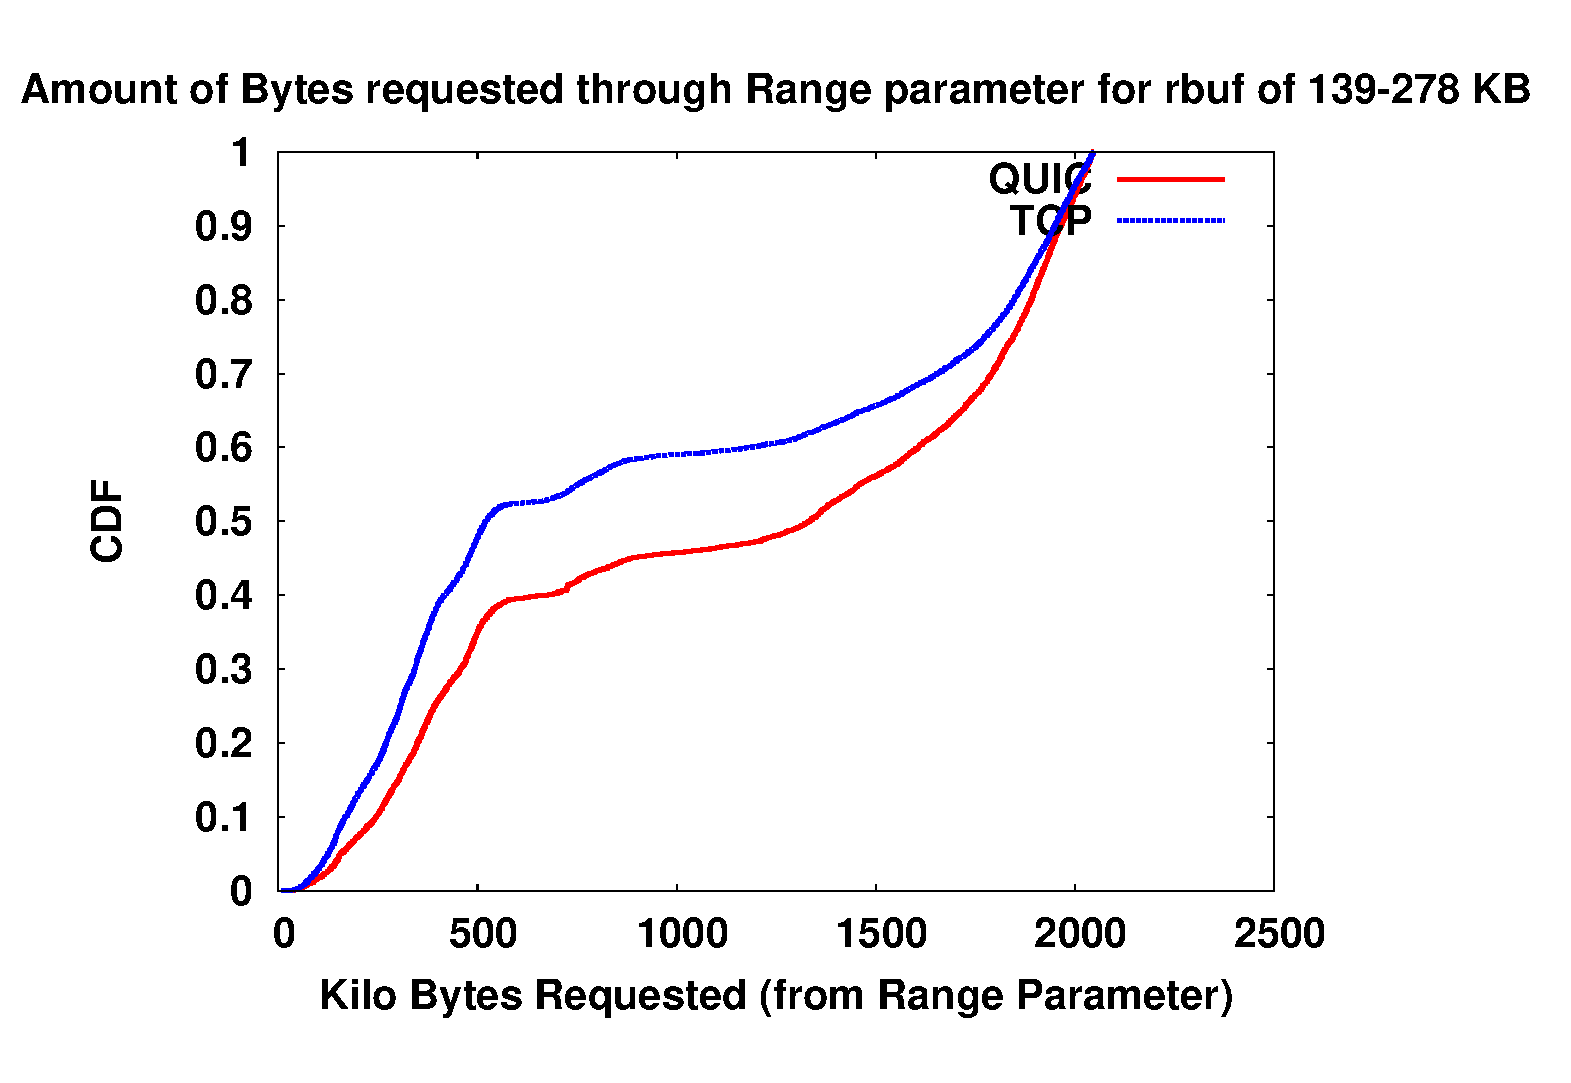
\includegraphics[width=0.9\linewidth]{img/CDF/plot_range_284734}
    \caption{CDF of range for rbuf 139-278KB}
    \label{fig:rabuf761856}
\end{figure}
\begin{figure}[!ht]
    \centering
    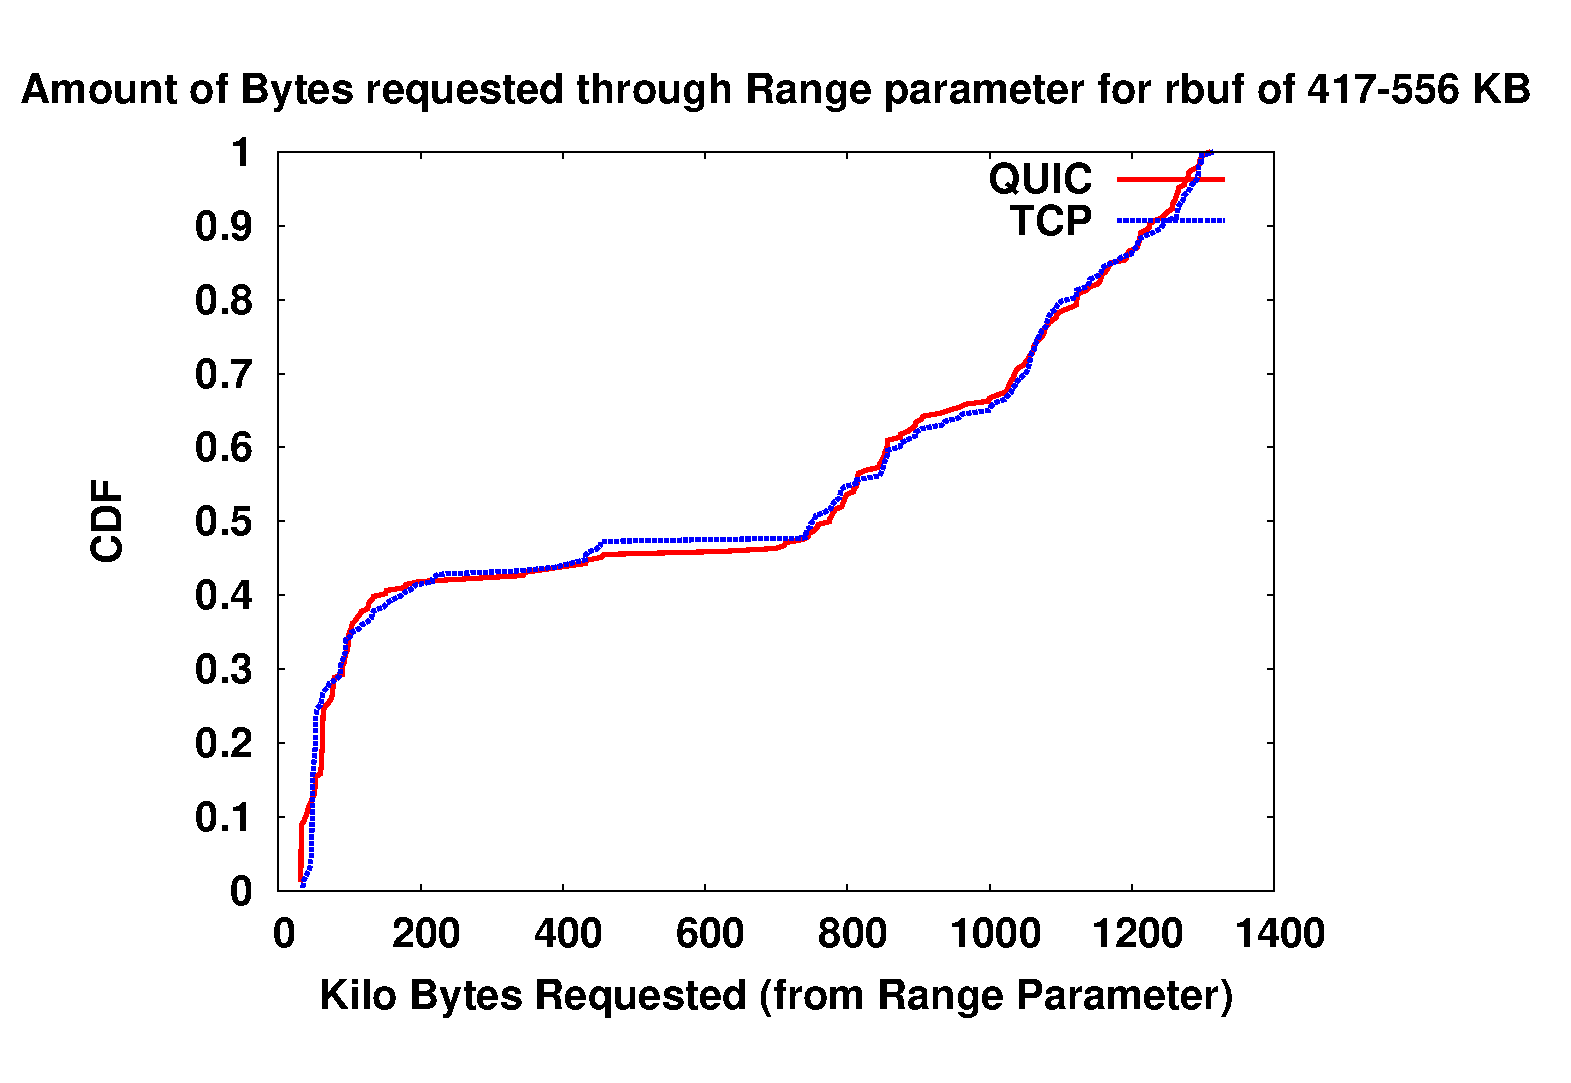
\includegraphics[width=0.9\linewidth]{img/CDF/plot_range_569468}
    \caption{CDF of range for rbuf 417-556KB}
    \label{fig:rabuf761}
\end{figure}
%\clearpage

